%%%%%%%%%%%%%%%%%%%%%%%%%%%%%%%%%%%%%%%%%
% Thesis 
% LaTeX Template
% Version 1.3 (21/12/12)
%
% This template has been downloaded from:
% http://www.latextemplates.com
%
% Original authors:
% Steven Gunn 
% http://users.ecs.soton.ac.uk/srg/softwaretools/document/templates/
% and
% Sunil Patel
% http://www.sunilpatel.co.uk/thesis-template/
%
% License:
% CC BY-NC-SA 3.0 (http://creativecommons.org/licenses/by-nc-sa/3.0/)
%
% Note:
% Make sure to edit document variables in the Thesis.cls file
%
%%%%%%%%%%%%%%%%%%%%%%%%%%%%%%%%%%%%%%%%%

%----------------------------------------------------------------------------------------
%	PACKAGES AND OTHER DOCUMENT CONFIGURATIONS
%----------------------------------------------------------------------------------------

\documentclass[12pt, a4paper, twoside]{Thesis} % Paper size, default font size and one-sided paper
\usepackage{pdfpages}
\usepackage{footnote}
\usepackage{graphicx}
\usepackage{xcolor}
\usepackage{xparse}
\usepackage{listings}
% \usepackage{subfig}
\usepackage{hyperref}
% \usepackage{subcaption}
\usepackage{caption}
% \usepackage{subcaption}
\graphicspath{{./Pictures/}} % Specifies the directory where pictures are stored
\usepackage[utf8]{inputenc}
\usepackage[square, numbers, comma, sort&compress]{natbib} % Use the natbib reference package - read up on this to edit the reference style; if you want text (e.g. Smith et al., 2012) for the in-text references (instead of numbers), remove 'numbers'
\NewDocumentCommand{\framecolorbox}{oommm}
 {% #1 = width (optional)
  % #2 = inner alignment (optional)
  % #3 = frame color
  % #4 = background color
  % #5 = text
  \IfValueTF{#1}
   {%
    \IfValueTF{#2}
     {\fcolorbox{#3}{#4}{\makebox[#1][#2]{#5}}}
     {\fcolorbox{#3}{#4}{\makebox[#1]{#5}}}%
   }
   {\fcolorbox{#3}{#4}{#5}}%
 }
\hypersetup{urlcolor=black, colorlinks=true} % Colors hyperlinks in blue - change to black if annoying
\title{\ttitle} % Defines the thesis title - don't touch this

\begin{document}
% \mainmatter
% ### FrontMATTER
% \frontmatter 


% Use roman page numbering style (i, ii, iii, iv...) for the pre-content pages

\setstretch{1.3} % Line spacing of 1.3

% Define the page headers using the FancyHdr package and set up for one-sided printing
\fancyhead{} % Clears all page headers and footers
\rhead{\thepage} % Sets the right side header to show the page number
\lhead{} % Clears the left side page header

\pagestyle{fancy} % Finally, use the "fancy" page style to implement the FancyHdr headers

\newcommand{\HRule}{\rule{\linewidth}{0.5mm}} % New command to make the lines in the title page

% PDF meta-data
\hypersetup{pdftitle={\ttitle}}
\hypersetup{pdfsubject=\subjectname}
\hypersetup{pdfauthor=\authornames}
\hypersetup{pdfkeywords=\keywordnames}

%----------------------------------------------------------------------------------------
%	TITLE PAGE
%----------------------------------------------------------------------------------------

\begin{titlepage}
\begin{center}

\textsc{\LARGE Saarland University}\\[1.5cm] % University name
\textsc{\Large Master's Thesis}\\[0.5cm] % Thesis type

% #### HORIZONTAL LINE 1 ####
\vspace{1cm}
% \HRule \\[0.6cm] % Horizontal line
{\huge \bfseries Robustness Analysis of Selenium test-suites}\\[0.4cm] % Thesis title
\vspace{1cm}
% #### HORIZONTAL LINE 2 ####
% \HRule \\[1.3cm] % Horizontal line
\begin{center}
\emph{Submitted by:}\\
{Aditya Nisal} 
\end{center}
\vspace{2cm}
\begin{minipage}{0.4\textwidth}
\begin{flushleft} 
\emph{Supervisor:}\\
{Dr. Andreas Zeller} % Author name - remove the \href bracket to remove the link

\end{flushleft}
\end{minipage}
\begin{minipage}{0.4\textwidth}
\begin{flushright} 
\emph{Advisor:} \\
{Andreas Rau} % Supervisor name - remove the \href bracket to remove the link  
\end{flushright}
\end{minipage}\\[1cm]


\begin{center}
\emph{Reviewers:}\\
{Dr. Andreas Zeller}\\
{Dr. Andreas Zeller}
\end{center}

\vspace{1.5cm}
\large \textit{Submitted in partial fulfilment of the requirements\\ for M.Sc. Computer and Communication technology}\\[0.3cm] % University requirement text
\textit{at}\\[0.4cm]
Software Engineering Chair \\Saarland University\\[1cm] % Research group name and department name
 
{\large \today}\\[1cm] % Date
%\includegraphics{Logo} % University/department logo - uncomment to place it
 
\vfill
\end{center}

\end{titlepage}

%----------------------------------------------------------------------------------------
% 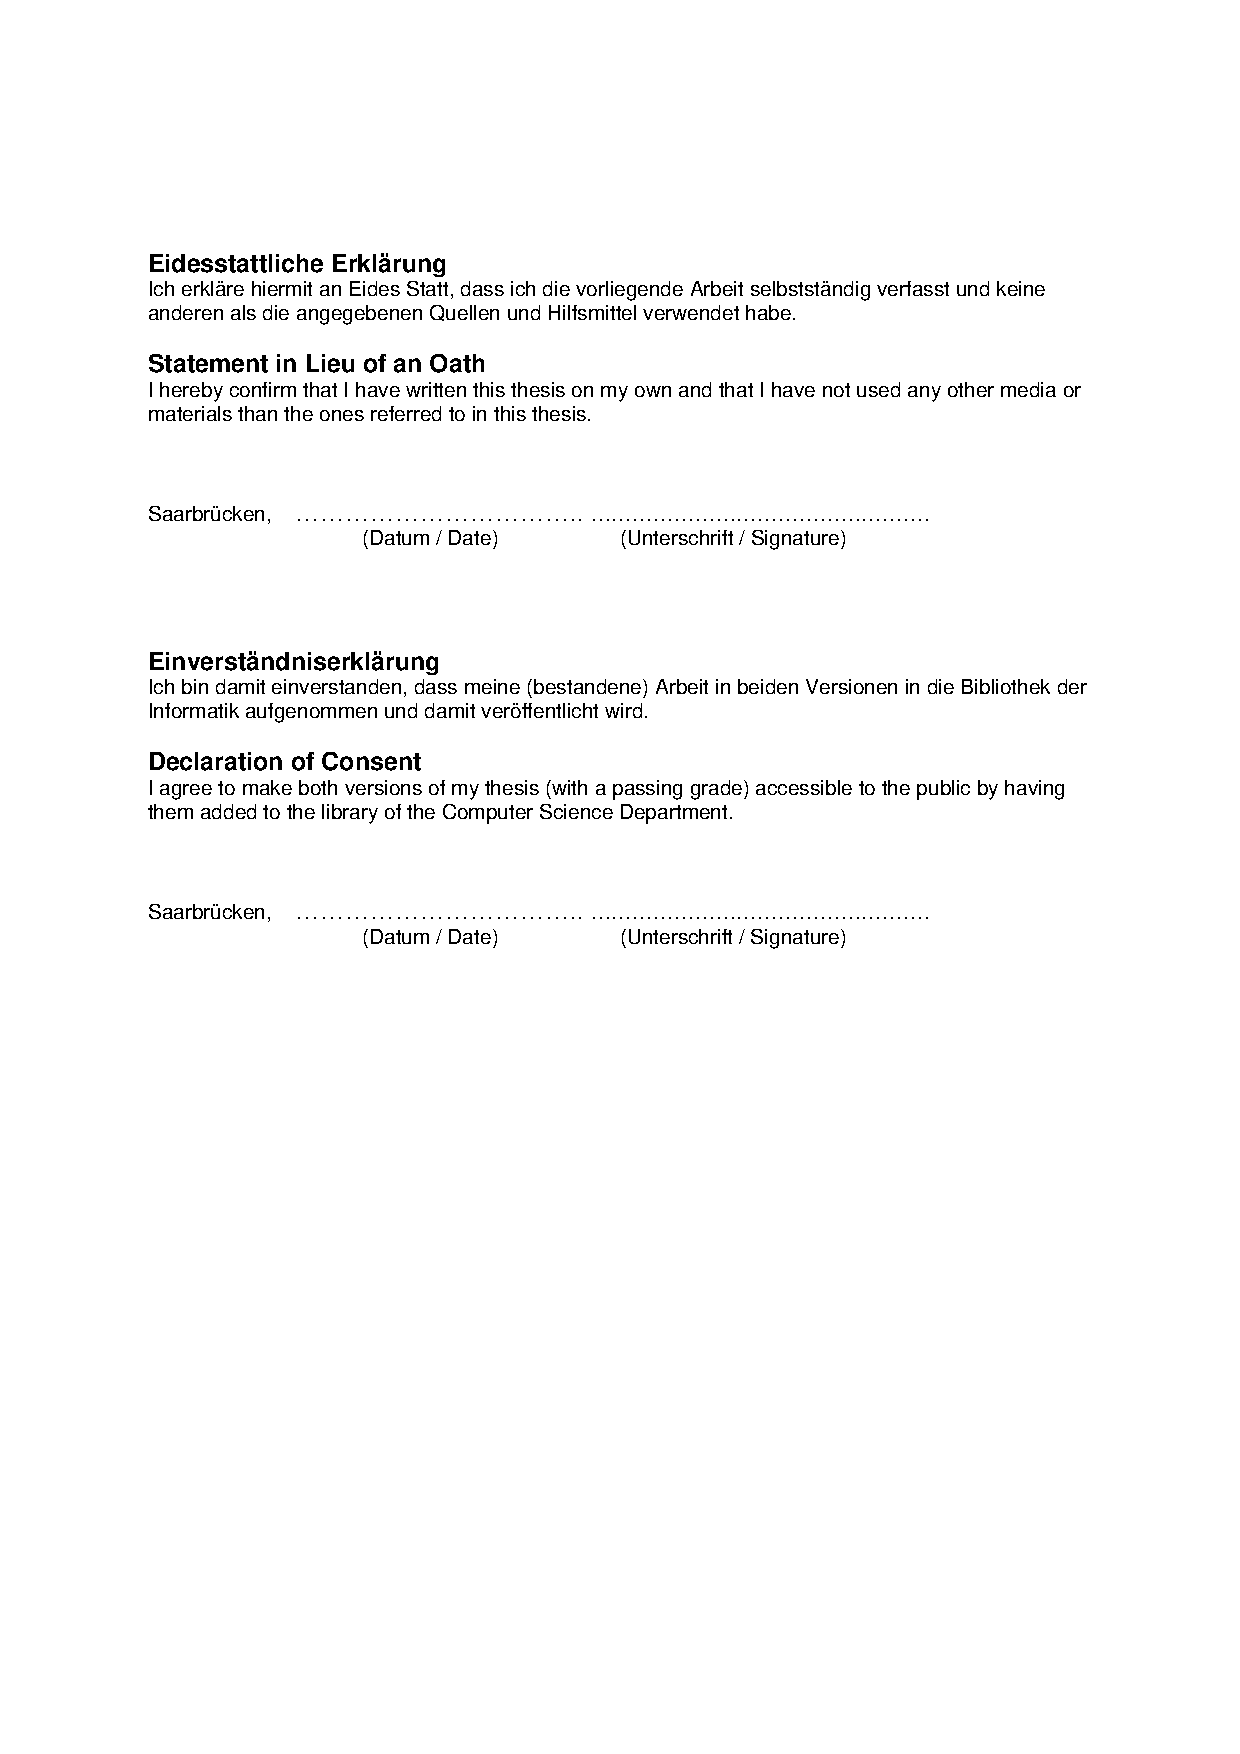
\includepdf[pages={-}]{Eidesst_Erkl_Abschlussarb_cuk.pdf}
%	DECLARATION PAGE
%	Your institution may give you a different text to place here


%----------------------------------------------------------------------------------------

% \Declaration{\vspace{1em}
\pagestyle{empty} 
\begin{center}
\Large\textbf{Eidesstattliche Erklärung} \\
\end{center}
\noindent
\begin{itemize}
\item
Ich erkläre hiermit an Eides Statt, dass ich die vorliegende Arbeit selbstständig verfasst und keine
anderen als die angegebenen Quellen und Hilfsmittel verwendet habe.
\item
Ich erkläre hiermit an Eides Statt, dass die vorliegende Arbeit mit der elektronischen Version
übereinstimmt. 
\end{itemize}
\begin{center}
\Large\textbf{Statement in Lieu of an Oath} \\
\end{center}
\noindent
\begin{itemize}
\item
I hereby confirm that I have written this thesis on my own and that I have not used any other media or
materials than the ones referred to in this thesis.
\item
I hereby confirm the congruence of the contents of the printed data and the electronic version of
the thesis. 
\end{itemize}
\begin{center}
\Large\textbf{Einverständniserklärung} \\
\end{center}
\noindent
\begin{itemize}
\item
Ich bin damit einverstanden, dass meine (bestandene) Arbeit in beiden Versionen in die Bibliothek der
Informatik aufgenommen und damit veröffentlicht wird.
\end{itemize}
\begin{center}
\Large\textbf{Declaration of Consent} \\
\end{center}
\noindent
\begin{itemize}
\item
I agree to make both versions of my thesis (with a passing grade) accessible to the public by having
them added to the library of the Computer Science Department.
\end{itemize}
\vspace{2cm}
Saarbrücken, $\rule{3cm}{0.15mm}$\hspace{4cm}$\rule{5cm}{0.15mm}$ \newline
\hspace*{2.5cm}(Datum / Date) \hspace{4cm}(Unterschrift / Signature)
% \addtocontents{toc}{\vspace{1em}} % Add a gap in the Contents, for aesthetics

% Eidesstattliche Erklärung
% Ich erkläre hiermit an Eides Statt, dass ich die vorliegende Arbeit selbstständig verfasst und keine
% anderen als die angegebenen Quellen und Hilfsmittel verwendet habe.
% Statement in Lieu of an Oath
% I hereby confirm that I have written this thesis on my own and that I have not used any other media or
% materials than the ones referred to in this thesis.
% Saarbrücken, …………………………….. ………………………………………….

%  (Datum / Date) (Unterschrift / Signature)
% Einverständniserklärung
% Ich bin damit einverstanden, dass meine (bestandene) Arbeit in beiden Versionen in die Bibliothek der
% Informatik aufgenommen und damit veröffentlicht wird.
% Declaration of Consent
% I agree to make both versions of my thesis (with a passing grade) accessible to the public by having
% them added to the library of the Computer Science Department.
% Saarbrücken, …………………………….. ………………………………………….
%  (Datum / Date) (Unterschrift / Signature)
 
% Signed:\\
% \rule[1em]{25em}{0.5pt} % This prints a line for the signature
 
% Date:\\
% \rule[1em]{25em}{0.5pt} % This prints a line to write the date
% }

\clearpage % Start a new page

%----------------------------------------------------------------------------------------
%	QUOTATION PAGE
%----------------------------------------------------------------------------------------

% \pagestyle{empty} % No headers or footers for the following pages

% \null\vfill % Add some space to move the quote down the page a bit

% \textit{``Thanks to my solid academic training, today I can write hundreds of words on virtually any topic without possessing a shred of information, which is how I got a good job in journalism."}

% \begin{flushright}
% Dave Barry
% \end{flushright}

% \vfill\vfill\vfill\vfill\vfill\vfill\null % Add some space at the bottom to position the quote just right

% \clearpage % Start a new page

%----------------------------------------------------------------------------------------
%	ABSTRACT PAGE
%----------------------------------------------------------------------------------------

% \addtocontents{toc}
% Add the "Abstract" page entry to the Contents
\abstract{\vspace{1em} % Add a gap in the Contents, for aesthetics

The Thesis Abstract is written here (and usually kept to just this page). The page is kept centered vertically so can expand into the blank space above the title too\ldots
}

\clearpage % Start a new page

% ----------------------------------------------------------------------------------------
% 	ACKNOWLEDGEMENTS
% ----------------------------------------------------------------------------------------

% \setstretch{1.3} % Reset the line-spacing to 1.3 for body text (if it has changed)

\acknowledgements{\vspace{1em} % Add a gap in the Contents, for aesthetics
\setcounter{page}{4}
The acknowledgements and the people to thank go here, don't forget to include your project advisor\ldots
}
\clearpage % Start a new page

%----------------------------------------------------------------------------------------
%	LIST OF CONTENTS/FIGURES/TABLES PAGES
%----------------------------------------------------------------------------------------

\pagestyle{fancy} % The page style headers have been "empty" all this time, now use the "fancy" headers as defined before to bring them back

\lhead{\emph{Contents}} % Set the left side page header to "Contents"
\tableofcontents % Write out the Table of Contents

\lhead{\emph{List of Figures}} % Set the left side page header to "List of Figures"
\listoffigures % Write out the List of Figures

\lhead{\emph{List of Tables}} % Set the left side page header to "List of Tables"
\listoftables % Write out the List of Tables

%----------------------------------------------------------------------------------------
%	ABBREVIATIONS
%----------------------------------------------------------------------------------------

% \clearpage % Start a new page

% \setstretch{1.5} % Set the line spacing to 1.5, this makes the following tables easier to read

% \lhead{\emph{Abbreviations}} % Set the left side page header to "Abbreviations"
% \listofsymbols{ll} % Include a list of Abbreviations (a table of two columns)
% {
% \textbf{LAH} & \textbf{L}ist \textbf{A}bbreviations \textbf{H}ere \\
% %\textbf{Acronym} & \textbf{W}hat (it) \textbf{S}tands \textbf{F}or \\
% }

%----------------------------------------------------------------------------------------
%	PHYSICAL CONSTANTS/OTHER DEFINITIONS
%----------------------------------------------------------------------------------------

% \clearpage % Start a new page

% \lhead{\emph{Physical Constants}} % Set the left side page header to "Physical Constants"

% \listofconstants{lrcl} % Include a list of Physical Constants (a four column table)
% {
% Speed of Light & $c$ & $=$ & $2.997\ 924\ 58\times10^{8}\ \mbox{ms}^{-\mbox{s}}$ (exact)\\
% % Constant Name & Symbol & = & Constant Value (with units) \\
% }

%----------------------------------------------------------------------------------------
%	SYMBOLS
%----------------------------------------------------------------------------------------

% \clearpage % Start a new page

% \lhead{\emph{Symbols}} % Set the left side page header to "Symbols"

% \listofnomenclature{lll} % Include a list of Symbols (a three column table)
% {
% $a$ & distance & m \\
% $P$ & power & W (Js$^{-1}$) \\
% % Symbol & Name & Unit \\

% & & \\ % Gap to separate the Roman symbols from the Greek

% $\omega$ & angular frequency & rads$^{-1}$ \\
% % Symbol & Name & Unit \\
% }

%----------------------------------------------------------------------------------------
%	DEDICATION
%----------------------------------------------------------------------------------------

% \setstretch{1.3} % Return the line spacing back to 1.3

% \pagestyle{empty} % Page style needs to be empty for this page

% \dedicatory{For/Dedicated to/To my\ldots} % Dedication text

% \addtocontents{toc}{\vspace{2em}} % Add a gap in the Contents, for aesthetics

%----------------------------------------------------------------------------------------
%	THESIS CONTENT - CHAPTERS
%----------------------------------------------------------------------------------------

% \mainmatter % Begin numeric (1,2,3...) page numbering

\pagestyle{fancy} % Return the page headers back to the "fancy" style

% Include the chapters of the thesis as separate files from the Chapters folder
% Uncomment the lines as you write the chapters

\chapter{Introduction} % Main chapter title


\label{Chapter1} % For referencing the chapter elsewhere, use \ref{Chapter1} 

\lhead{Chapter 1. \emph{Introduction}}
% \HRule \\[0cm]


1. Why use state-models, why not just check stack trace? 
-> Tells us at which step failure occured. 
- tells us the extent to which certain functionality is covered. 
- don't write large tests, just do small ones. Often, when functional tests fail, they tell you something failed, but they don't tell you what failed. The shortest possible functional tests help reduce the scope of where a problem can be. Other benefits of short tests are they're easier to read and easier to write.

RQ2 - remind people that you're doing it at test level. How each test reacts as a combination of all building blocks.

-- Reasons behind NoSuchElement etc if it happens randomly: 
1. Failed to invoke a constructor of class 
2. Timeout: Explicit wait is set and no element is found then it gives timeout error
3. 

\subsubsection*{Background}
Add implicitWait
\subsubsection*{RQ1 tips}
1. Discuss how each test suite is at the end
2. Discuss page objects
3. Extra long Xpaths
4. Test dependencies Esp. moodle
5. Discuss that AMO,Fireplace,Bedrock all have small tests. Jenkins creates huge slaves, memory allocation, multitude of Sendkeys. Jenkins uses Guice, Jenkins has long running jobs, creation of big files, Moodle has lots of form data validation but all locators are relative 
6. Discuss tests which were added or removed 
7. Look and feel does not affect robustness 


\newpage
In recent years, web applications have become a popular alternative to traditional desktop applications.
% To access a web application, the end-user is only required to maintain a functioning web-browser, whereas the application vendor can deploy and update the application independent of end-users’ system configurations. 
During the evolution of a web application, it is repeatedly modified to add new functionalities, fix bugs or adapt the GUI (Graphical User Interface) to improve the user experience. After such modifications, it is not uncommon to encounter side effects manifested in the form of new bugs or re-emergence of old bugs. Such side effects usually occur as a result of changing system or component configurations, improper version control, applying incorrect or incomplete bug fixes, etc. and can therefore negatively affect the quality of the existing functionality. 

To ensure that after such modifications the application maintains its quality and still fulfills the existing specifications, regression tests are performed on the Application Under Test (henceforth referred as AUT). Software developers typically re-run the existing test-suite \cite{rothermel2001prioritizing}, \cite{elbaum2000prioritizing} along with a set of test inputs and test \textit{oracles} — mechanism to assess the test output \cite{1240304}, on a newly developed version. This process ensures that the code and functionality carried over from older version behaves as expected.

Depending upon the development cycle, project size and available resources, regression tests can be performed at different abstraction levels, commonly as \textit{unit, integration} and \textit{system testing} \cite{Mpezze}. Unit tests are intended to test small pieces or modules of code, such as functions and classes, whereas integration tests are aimed to test the system as composition of different components. System level tests are performed at higher abstraction level similar to integration tests, however, their goal is to check whether the software meets the functional specifications. 

Intuitively, in case of web applications the regression testing can be done at the GUI level, since majority of web applications’ functionality is accessed through this layer. In traditional sense, regression testing at GUI level abstracts away finer grained internal details by treating the AUT as a black-box. Such testing helps developers to identify the undesired changes in required functionality of the application.
% , since the GUI might have changed significantly while the underlying application has not. 

Dallmeier et al. \cite{webmate} presented the tool \texttt{webmate} for testing web 2.0 applications. To this date, \texttt{webmate} primarily functions as a cross-browser compatibility testing tool and supports different browsers and platforms. It can systematically explore the AUT by executing automated GUI tests and detect functional as well as GUI level differences in the AUT. 

As the application size increases, the possible combinations of inputs increase along with GUI exploration paths. Hence, GUI testing becomes more complicated as a typical GUI test involves multiple sequential operations because certain functionalities are only accessible through a series of GUI events.
% For example, to purchase an item in a typical e-commerce web application a user would need to perform sequential events such as login, add product to cart, fill payment details and finally checkout. This flow can vary depending on additional functionality such as purchasing pre-selected products, favourites etc. 
% As the possible number of paths and sequences increases, generating test inputs and applying test oracles becomes more difficult and costly. 
% Additionally, different browsers implement different technologies which might result in varied rendering of the GUI, making regression testing more complicated.

To reduce the costs incurred with manual testing, many developers choose to automate regression tests using Selenium \cite{websiteSelenium} framework. The Selenium project provides the \texttt{webdriver} API (Application Programming Interface) to test web 2.0 applications. The API \textit{drives}, i.e. controls, the web browser in a manner that it emulates all possible user interactions with the application, such as clicks, form-inputs, file uploads etc. 
% Figure \ref{code1} illustrates 
As an example,\footnote{A similar depiction of the problem has also been done by Leotta et al. \cite{leotta2013comparing}} to test the \textit{login} functionality of AUT as depicted in Figure \ref{fig:a}, a \texttt{webdriver} based test \texttt{"loginTest"} would navigate to the homepage of AUT, fill the \textit{username} and \textit{password} fields and finally click the \textit{`Login'} button using the hyperlink text ``Login'' as following (in Java):
\begin{small}
\texttt{driver.findElement(By.linkText("Login")).click()}
\end{small}


\begin{figure}[ht!]
\centering     %%% not \center
\subfigure[AUT version $V_{0}$]{\label{fig:a}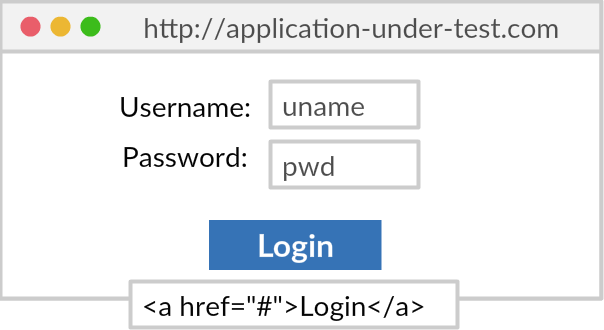
\includegraphics[width=5.6cm,height=2.8cm]{./Figures/newlogin}}
\vspace{-2mm}\subfigure[AUT version $V_{1}$]{\label{fig:b}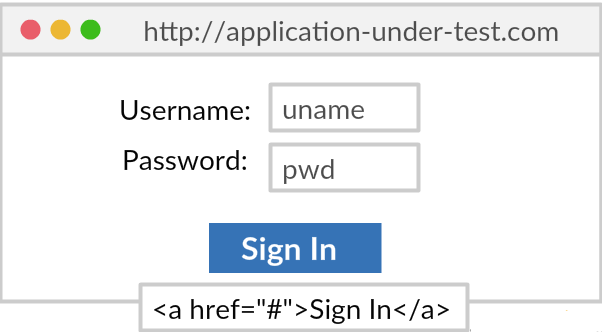
\includegraphics[width=5.6cm,height=2.8cm]{./Figures/newsignin}}
\caption{Visual comparison of version $V_{0}$ and $V_{1}$ of AUT}
\label{fig:loginTest}
\end{figure} 
% \begin{minipage}{0.45\textwidth}
% % \begin{figure}
% 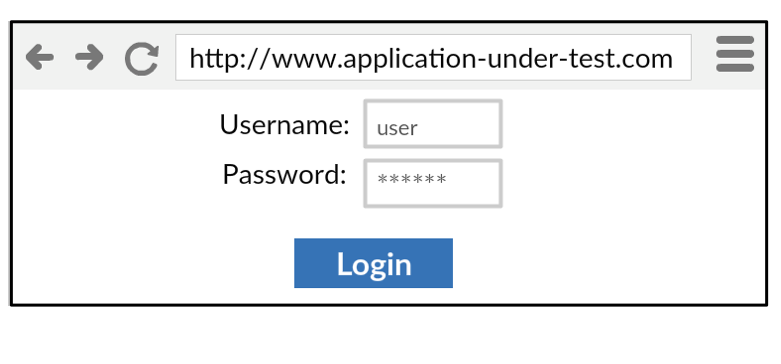
\includegraphics{./Figures/Login-button}
% \caption{Login}
% \label{fig:loginTest}
% % \end{figure}
% \end{minipage}%



% \begin{minipage}{0.5\textwidth}
% \begin{center}

% \begin{scriptsize}
% \lstset{
%   basicstyle=\ttfamily,
%   columns=fullflexible,
%   keepspaces=true,
% %   frame=none,
% }
% % \verb|basicstyle=\ttfamily, columns=fullflexible, keepspaces=true|
  
% \begin{lstlisting}[caption=Login test,label=code1]
% public void loginTest(){
% driver.get("http://www.application-under-test.com");
% driver.findElement(By.id("uname")).sendKeys("user");
% driver.findElement(By.id("pwd")).sendKeys("passwd");
% driver.findElement(By.linkText("Login")).click();
% }
% \end{lstlisting}
% \end{scriptsize} 
% \end{center}
% % \end{minipage}%

Compared to manual tests, Selenium tests can be run automatically and repeatedly. Typically, such tests can be combined with Continuous Integration tools to be run after the code changes are pushed to the version control repository. When AUT evolves from version $V_{0}$ to a newer version $V_{1}$, existing Selenium tests are executed on $V_{1}$. Ideally, if one or more tests executed successfully on $V_{0}$ fail to achieve the same result on $V_{1}$, the tests have found the possible \textit{software regressions} in the AUT. This approach in reality relies heavily on the quality and robustness of the existing tests. Intuitively, robustness of Selenium tests implies their reliability and effectiveness to achieve the same functional coverage across different versions of the AUT. 

% """However, as the web application continues to evolve, robustness of Selenium tests decreases over time."""

As the web application continues to evolve, existing Selenium tests might not achieve the same functional coverage as they do for the version the tests are originally written for. Consider the aforementioned example of \texttt{loginTest} where the outcome of code changes in AUT results in changing the display text of \textit{`Login'} button to ``Sign In'' in version $V_{1}$. When \texttt{loginTest} is re-run on $V_{1}$, it is unable to locate the \textit{`Login'} button since the hyperlink text ``Login'' is changed to ``Sign in''. As a result, \texttt{loginTest} is broken and the desired functional coverage is not achieved -- unless this fragile (non-robust) test is repaired. If Selenium tests are not robust and resilient enough as the AUT evolves, desired functional coverage is not achieved and regression testing becomes inefficient.


Unfortunately, such situations are not uncommon in agile development environments which involve frequent changes in the AUT \cite{martin2003agile}. The reasons for decreasing robustness and failures of Selenium tests includes changed functionality, modified GUI element locators, changed structural markup and timing issues etc. To repair the fragile tests, developers need to invest time and efforts to analyze the functionality changes, identify test failures manually and maintain such test-suites. In other words, when the AUT changes frequently, fragile tests need to be repaired repeatedly to cope with these changes, which can be an expensive and time consuming task for developers. 

As Selenium tests directly depend upon GUI element locators for locating desired object (e.g. a button) in the AUT, selection strategy for locating GUI elements plays vital role in dictating the robustness of Selenium tests. If a test implements structure based locators such as layout-dependent \texttt{xpath} expressions to find relative position of an element on the web page, slight changes in the structure of the web page can diminish the robustness of the test. Such situations can arise upon renaming the display hyperlink text (Figure \ref{fig:b}) or changing the HTML structure, such as changing the structure of the page through \texttt{<div>} tags. On the contrary, element locators such as unique element \texttt{id} attributes are not affected by such changes and can be used to write robust tests. 

Leotta et al. \cite{leotta2015using} present an algorithm for selecting reliable \texttt{xpath} locators from a set of absolute and relative \texttt{xpath} expressions for the AUT. Another study by Leotta et al. \cite{leotta2013comparing} compares the effort required to maintain \texttt{id, xpath} and \texttt{link text} locators. Nevertheless, these approaches cover only a subset of available element locators and measure the stability of Selenium tests in terms of the effort required to maintain these locators. Apart from the GUI element locators, the design and composition of tests such as the number of actions performed by the tests, mechanisms implemented to deal with timing issues (e.g.\smallskip implementing \texttt{wait} commands) also dictate the robustness of Selenium tests. 

% Robustness of Selenium tests can be defined in terms of their stability and effectiveness to achieve the same functional coverage across different versions of the AUT. 
% The reasons for decreasing robustness and failures of Selenium tests can include changed functionality, modified GUI element locators and changed structural markup, timing issues etc. 
% Such non-robust tests exhibiting decreased functional coverage are unsuitable for regression testing unless these tests are repaired. In order to modify such tests, developers need to invest time and efforts to analyze the undesired functionality changes, identify test failures manually and maintain such test-suites.

% In other words, if the Selenium tests are not robust enough, the regression testing is likely to be ineffective.

Considering the current state-of-the-art technologies to the best of my knowledge, thus far there has been no direct research in the area of assessing the robustness of Selenium tests over the version history of the web applications. Such analysis would help developers to understand the common reasons behind varying robustness of Selenium regression tests and write more robust tests. The primary goal of this thesis is to measure the robustness of Selenium test-suites over the version history of web applications and identify the factors affecting robustness. 

% \begin{figure}
% \begin{subfigure}[b]{0.31\textwidth} 
% 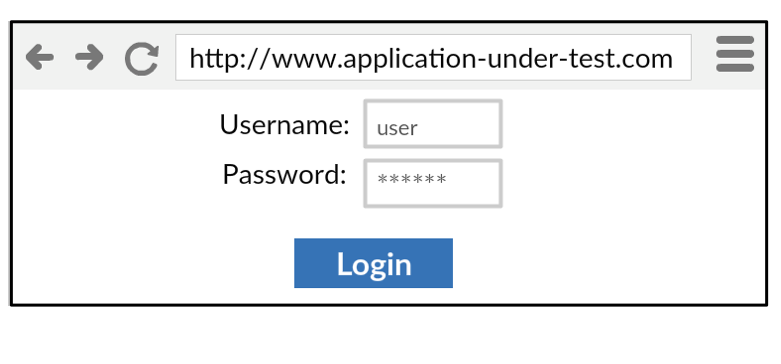
\includegraphics[width=7cm, height=3.2cm]{./Figures/Login-button}
% \caption{First subfigure}\label{fig:1a}
% \end{subfigure}
% \hspace*{\fill} % separation between the subfigures
% \begin{subfigure}{0.31\textwidth}
% 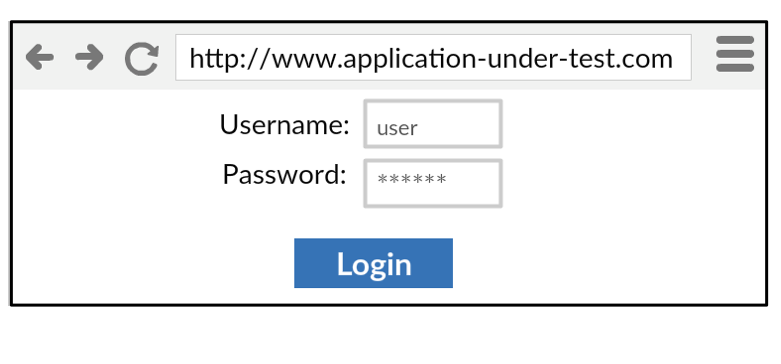
\includegraphics[width=7cm, height=3.2cm]{./Figures/Login-button}
% \caption{Second subfigure}\label{fig:1b}
% \end{subfigure}
% \caption{A figure that contains three subfigures}\label{fig:1}
% \end{figure}

% \subcaptionbox{The left subfigure with a long caption spanning several lines and some more text}%
%   [.4\linewidth]{\includegraphics[height=2cm]{example-image-a}}
%% THIS ONE WORKS !!!!!

% \begin{figure}
% 	\centering	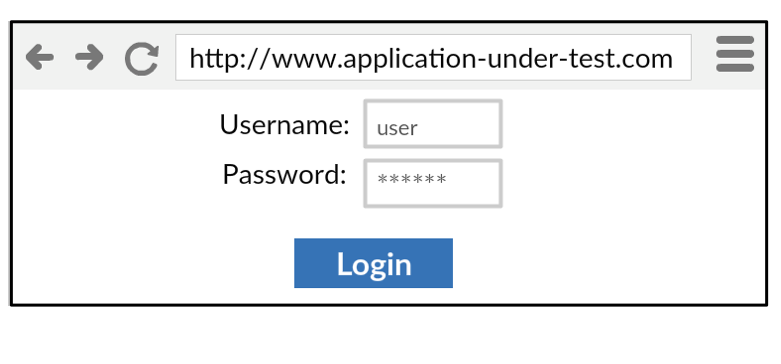
\includegraphics [width=7cm, height=3.2cm]{./Figures/Login-button}
% 	\caption{Login functionality of AUT}
% 	\label{fig:loginTest}
% \end{figure} 


The first step is to formally establish and define \textit{robustness} in terms of a measurable metric. A test can be marked as ``passed'' in the output logs but still land on different web pages of the AUT. Such test might not have covered the same functionality and cannot be considered robust. Furthermore, to identify the factors behind the varying robustness of Selenium tests, as mentioned earlier, a set of metrics has to be developed (Chapter \ref{Chapter3}). 

This thesis proposes the metric \textit{`robustness grade'} of a test which allows us to determine its effectiveness for regression testing. On a coarser level, \textit{`robustness grade'} of a test-suite can indicate its overall quality and suitability for regression testing. A high robustness can be another indication of the maintainability of the test-suite, since robust tests do not need to be repaired and maintained as frequently. If the proposed metrics are able to determine which factors impact robustness the most, developers can use these metrics to write more robust tests. This research aims to answer the following research questions:
\newline
{\bfseries RQ1} How robust are Selenium tests over time as the underlying application evolves?  \newline
{\bfseries RQ2} Is robustness correlated to the design and composition of the tests?\newline
{\bfseries RQ3} Which GUI element locator requires the least maintenance effort over time?\newline
{\bfseries RQ4} Can the robustness analysis improve current Selenium testing practices?\newline

% \\
% {\bfseries RQ1} How to determine the robustness of Selenium tests?
% {\bfseries RQ2} Is the change in robustness correlated to the changes of application’s structural elements?
% {\bfseries RQ4} Do tests with shorter execution traces tend to be more robust than tests with relatively longer traces?
% {\bfseries RQ5} Does same test input result in different GUI states of the AUT for different versions (\textit{reachability problem})?
% {\bfseries RQ6} Can the robustness analysis improve or assist current Selenium testing practices?
% {\bfseries RQ7} Reasons of failure behind test cases?
% {\bfseries RQ8} Size and complexity of test suite?
% \\

Figure \ref{fig:thesisoverview} depicts the setup required for performing the robustness analysis and answer aforementioned research questions. 
The first step is to select suitable testing candidates for this research and extract Selenium tests-suites from their test repositories. The approach is to deploy different versions of test candidates AUT and run automated Selenium regression tests on them. In the next step, Selenium tests are leveraged with the existing tool \texttt{webmate} \cite{webmate} to capture the application behavior in terms of behavioral state models. The \textit{states} of the state model represent the abstracted DOM (Document Object Model) states and \textit{transitions} represent actions executed on AUT. Such a state model allows us to compare the outcome of Selenium tests on different releases in comparison to the release for which the test-suite is written for. This step is essential for evaluating the functional behavior covered by the tests across different releases. Afterwards, \textit{`robustness grade'} is calculated for each test along with other metrics as defined in Chapter \ref{Chapter3}.\newline

\begin{figure}[h]
% [htbp]
	\centering	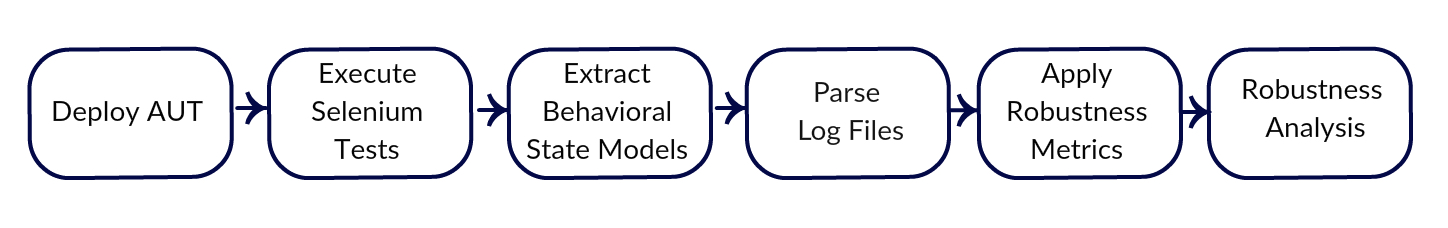
\includegraphics[width=\textwidth]{./Figures/thesisoverviewsmall.jpg}
%     [width=5cm, height=3cm]
% 		\rule{35em}{0.5pt}
	\caption{Setup required for the robustness analysis}
	\label{fig:thesisoverview}
\end{figure} 

This thesis is structured in following manner: Chapter 2 discusses the background terminologies. Chapter 3 discusses the research questions in detail and provides necessary implementation details. Chapter 4 presents the evaluation and results. Chapter 5 discusses threats to validity. Chapter 6 discusses conclusion and future
% \texttt{This section needs to be re-written}\newline
% \noindent This thesis is structured in following manner:
% \begin{itemize}
% \item Chapter 2 discusses the background terminologies
% \item Chapter 3 discusses the research questions in detail and provides necessary implementation details
% \item Chapter 4 presents the evaluation
% Approach and Evaluation : 20 pages
% Approach: Candidate selection, deployment, modifying selenium tests to fit to remotewebdriver, using sessionIDs to track, explaining how the entire grid works, extraction of state-models, comparison of GUI sequences, major minor versions,
% Evaluation: Experimental setup, test results, robustness metrics calculation, graphs, results
% For evaluating the approach and answer the research questions, the idea was to assess publicly available Selenium tests, in order to eliminate the possible bias introduced by writing one’s own Selenium tests as such are written from a single person’s design approach. In the same spirit, the presented model is tested on six different open source projects, from different domains as follows.
% \item Chapter 5 discusses threats to validity 
% \item Chapter 6 discusses conclusion and future work 
% \end{itemize}

 
\chapter{Background}
\label{Chapter2}
% Main chapter title
\lhead{Chapter 2. \emph{Background}}


This chapter introduces the background and terminology necessary to understand the concepts and methods presented in this thesis. Important terms are explained in corresponding sections.

As majority of web applications' functionality is accessed through the GUI layer, it becomes customary to test important functional use-cases on the AUT through the GUI layer. Section \ref{sec:AutomatedGUITesting} gives a brief insight into automated GUI testing mechanisms.

In recent years, Selenium\footnote{\url{http://www.seleniumhq.org/}} has been a popular browser test automation tool of choice among software developers and testers. Section\ref{sec:SeleniumTesting} gives the necessary background about Selenium framework, including its implementation techniques as well as salient features.

This research leverages existing Selenium tests to capture the behavior of the AUT in terms of finite state models. For this purpose, the tool \texttt{webmate}, presented by Dallmeier et al.\cite{webmate} has been used. By leveraging existing Selenium tests, \texttt{webmate} can systematically explore the AUT to extract its behavioral usage model by implementing state-abstraction for comparing similar GUI states of the AUT. Further details about \texttt{webmate} are discussed in Section \ref{sec:WebMate}

Section \ref{sec:Statistical} presents the statistical background required to analyze the results and apply the evaluation metrics, as presented in Chapter \ref{Chapter6}.

\section{Automated GUI Testing}
\label{sec:AutomatedGUITesting}
As mentioned in Section 1, testing web applications at GUI level abstracts away finer grained internal details and helps developers to identify the undesired functionality changes in the AUT.  In comparison to traditional command-line applications or Application Programming Interfaces (APIs), automated GUI testing of modern web 2.0 applications built with multiple languages, platforms and server-side technologies poses new challenges in the areas of test-input generation, test-output verification and state space exploration.

To begin with, automatically generating and selecting inputs for a GUI is difficult since depending upon the type of the application, different applications might require specific combinations of inputs and values. 
Current practices for automated test input generation include techniques such as symbolic execution\cite{Ganovetal}, using random input generation\cite{godefroid2005dart} or search based techniques\cite{gross2012search}. However, automated input generation is not trivial for a web applications, since the GUI test automation tool needs to be aware of the context of the AUT. Although test inputs can be generated using functional specifications, concrete specifications along with different input combinations may not be available in practice and desired functional coverage of the AUT is not achieved. Thus in many cases, input generation is often left to the test developer to explore the desired states of the AUT hidden behind input forms and elements.

In addition, even in cases when a testing tool can generate different input combinations automatically, it still needs to verify the correct behavior of the AUT. This is usually done by applying appropriate test assertions and oracles on the test outputs\cite{Baresi:Oracles}. Mechanisms such as using Capture/replay tools\cite{joshi2006capture} require the tester to first manually capture the behavior of the AUT by performing different GUI-level events, recording them and storing the expected output as a part of the test-case. In the replay phase, recorded tests are replayed on the AUT and the output is checked against the captured textit{expected output} to assert the application behavior. Such approach requires manual effort to record each test and is not suitable for regression testing as every time the AUT changes, there is a need to re-record the tests in order to generate new expected outputs. 

Moreover, as the size of the AUT increases, the number of possible actions on the GUI increases exponentially. This is especially an issue in case of regression testing since as possible number of paths and sequences increases, covering the entire possible number of state space and executions becomes infeasible.

On the other hand, as opposed to the automated crawlers, humans possess the domain knowledge of the AUT required to generate valid test inputs and apply precise oracles on the test outputs, many developers often choose to identify the core functionality of the AUT and automate their regression tests using frameworks such as Selenium, as detailed in Section 2.2.

\section{Test automation using Selenium}
\label{sec:SeleniumTesting}
\subsection{Selenium WebDriver}
Selenium is a browser automation framework designed to automate the system testing of web applications. While the Selenium project offers a different set of tools depending upon the type of application, the  \texttt{webdriver}\footnote{\url{http://www.seleniumhq.org/projects/webdriver/}} project is of particular the interest for laying the foundation of this thesis. The \texttt{webdriver} project provides an API to test dynamic web 2.0 applications. 

The \texttt{webdriver} API supports various modern programming languages such as Java, Python, C\#, Ruby, PHP etc. by providing language level bindings along with a set of browser specific drivers. Figure \ref{fig:webdriverArchitecture} gives an overview of the architecture of Selenium \texttt{webdriver}.

The API \textit{drives} (controls) the browser in a manner that it emulates all possible end users interactions with the browser, such as clicks, form-inputs, drag-drops, file uploads etc. Selenium \texttt{webdriver} tests can thus explore the possible set of functionalities of the AUT. As an example, Snippet \ref{code1} tests the \textit{login} functionality of AUT as depicted in Figure \ref{fig:a}.
\begin{center}
\begin{scriptsize}
\centering
\lstset{
  basicstyle=\ttfamily,
  columns=fullflexible,
  keepspaces=true,
%   frame=none,
}
% \verb|basicstyle=\ttfamily, columns=fullflexible, keepspaces=true|
  
\begin{lstlisting}[caption=Login test,label=code1]
public void loginTest(){
driver.get("http://www.application-under-test.com");
driver.findElement(By.id("uname")).sendKeys("user");
driver.findElement(By.id("pwd")).sendKeys("passwd");
driver.findElement(By.linkText("Login")).click();
}
\end{lstlisting}
\end{scriptsize} 
\end{center}
 
\begin{figure}[h!]
\makeatletter 
% \renewcommand{\thefigure}{\@arabic\c@figure}
\makeatother
    \centering
  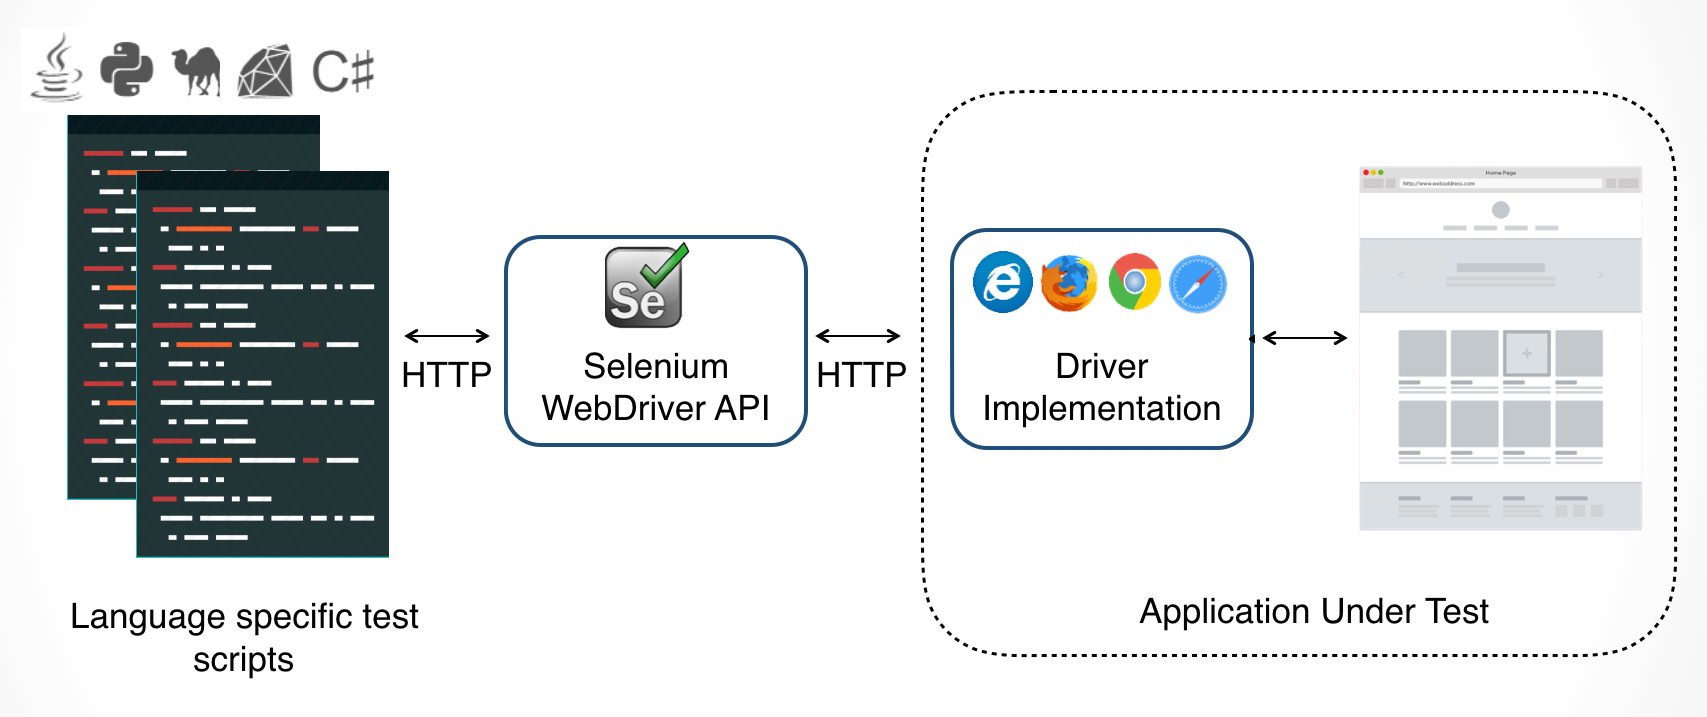
\includegraphics[width=5.5in,height=2.2in]{./Figures/webdriver_Archi}
  \caption{Selenium \texttt{webdriver} architecture}
  \label{fig:webdriverArchitecture} 
\end{figure}

The \texttt{webdriver} API communicates with the browser specific driver using a common wire protocol. The protocol transfers the test-commands written in language specific bindings to the browser specific driver in the form of UTF-8\footnote{\url{https://tools.ietf.org/html/rfc3629}} encoded JSON\footnote{\url{http://www.json.org/}} data. The API uses HTTP\footnote{\url{https://www.w3.org/Protocols/}} as a transport mechanism to transfer these commands to the driver and to return the response from the driver to the language specific code. 

Each browser specific driver implementation such as the \texttt{Firefox Driver}\footnote{\url{https://code.google.com/p/selenium/wiki/FirefoxDriver}} or the \texttt{RemoteWebDriver}\footnote{\url{https://code.google.com/p/selenium/wiki/RemoteWebDriver}} has its own mechanism for carrying out the above-mentioned communication. 

The \texttt{RemoteWebDriver} implementation provides the capability to run the Selenium tests against a remote machine. In essence, \texttt{RemoteWebDriver} is comprised of a client-server architecture, where client is the language specific test-case and and server is a simple Java servlet. The \texttt{RemoteWebDriver} servlet acts as a multiplexer, by connecting the client to the specific browser(s) and system configurations requested by the client. The browser and other configurations are provided in terms of capabilities, via command-line or directly from the language specific code. \\

\noindent 
Following example illustrates the communication between the language specific test-commands (Java in this case) and the \texttt{RemoteWebDriver} through \texttt{webdriver} API :
\begin{enumerate}
\item The client (test-script) requests the URL of the AUT. 
\begin{verbatim}
driver.get("http://www.application-under-test.com");
\end{verbatim}
\item This command is translated as a JSON object to be transferred using the wire protocol as following: 
\begin{verbatim}
{"url": "http://www.application-under-test.com" }
\end{verbatim}
\item The JSON object is then sent over HTTP (using POST\footnote{\url{http://tools.ietf.org/html/rfc7231\#section-4.3.3}} request in this case). To identify and associate each request/response session uniquely to the session-specific commands, \texttt{webdriver} uses a unique handle in terms of the \textit{SessionId}
\begin{verbatim}
HTTP Method : POST, Path: session/{session-id}/url
\end{verbatim}
The resultant URL is :
\begin{verbatim}
http://localhost:7055/hub/session/{session-id}/url
\end{verbatim}
\end{enumerate}

In order to locate GUI elements such as input forms, buttons, checkboxes etc. in the DOM (Document Object Model), Webdriver specifies "Find Element" and "Find Elements" methods for locating a single element and a list of elements, respectively. Each language specific binding has its own command to invoke these methods by providing the UI locator object, such as the css selector or xpath expression. The the element locator strategies are listed in TABLE XXX. As we will see in CHAPTER XXX ROBUSTNESS, influence of these UI locator strategies is discussed 
% (https://w3c.github.io/webdriver/webdriver-spec.html#sessions)

\section{WebMate}
\label{sec:WebMate}
WebMate is a system-level automated testing and analysis framework. It can leverage existing Selenium tests in order to remote control the browser to interact with the dynamic web 2.0 applications involving JavaScript and Ajax elements. By doing so, it can systematically explore the AUT in order to extract its behavioral usage-model. To do so, it implements state abstraction in order to distinguish similar GUI states of the AUT. The usage model is a finite state automaton, which captures the exploration graph of the possible ways to interact with the AUT. The states of the behavioral model correspond to different states of the GUI, connected by transitions corresponding to different interactions with the AUT. 
To this date, WebMate primarily functions for checking cross-browser compatibility. It can detect functional as well as GUI differences across the browsers. WebMate is able to identify the GUI elements and compare their positions, sizes and inconsistencies across the GUIs to generate a report visualizing the differences. Moreover, WebMate makes it possible to recognize functional differences (e.g. missing button) by comparing the usage models and presenting the XPath representation of the changed element

\section{Statistical Background}
\label{sec:Statistical}
% \chapter{Related Work} % Main chapter title

\label{Chapter3} % For referencing the chapter elsewhere, use \ref{Chapter1} 

\lhead{Chapter 3. \emph{Related Work}} 
\chapter{Robustness of Selenium Tests} % Main chapter title

\label{Chapter4} % For referencing the chapter elsewhere, use \ref{Chapter1} 

\lhead{Chapter 4. \emph{Robustness of Selenium Tests}}

Selenium tests are robust if these tests are able to cover same functionality for different versions of the AUT. Consequently, given tests are not robust if they do not achieve the same behavioral coverage as they do for the version the tests are originally written for.

\section{Factors responsible for varying robustness:}
\label{sec:RobustnessFactors}
As mentioned in Chapter XXXX, the stability and effectiveness of Selenium tests decreases over time across the regression cycles. In this section, we attempt to acknowledge the attributes of varying robustness of Selenium tests and further recognize the reasons behind the test failures. 

\subsection{Undesired functionality changes:}
\label{sec:FuncChanges}
Selenium tests are not robust if they are unable to cover the expected behavior when certain functionality is modified or removed as a result of regression changes. Such modified functionality might not be covered by the existing tests unless they are modified, since the same test inputs can lead to the behavior different than expected.

\subsection{Modifying structural markup and GUI elements:}
\label{sec:GUIChanges}
GUI level modifications and changes can affect the state changing elements such as clickable objects, buttons, forms etc. Thus, Selenium tests can be broken if the manner in which a functionality can be accessed (e.g. via clickable elements) is modified. Moreover, when content such as the element ‘id’, ‘CSS-selectors’ or ‘Xpath’ attributes etc. are modified or incorrectly selected, the test cases might be unable to find the object on the page as these attributes can no longer be valid.

\subsection{Page loading times and timing issues:}
\label{sec:PageLoadingTimes}
Depending upon various factors, different pages and page-objects of an AUT can load with different speeds. If such pages and objects do not load properly or have poor timing issues, the Selenium API can be unable to find them. The API returns an element as soon as it is available in the DOM. However, due to the timing issues the elements might not yet be ready to interact with. Such issues can result in sporadic failures during the test execution, making the tests less robust. We further identify the factors responsible for timing issues as follows: 

\begin{itemize}
  \item Server side requests such as Ajax and JavaScript calls can contribute towards random loading times. Recognizing when such calls are finished can be intricate for Selenium WebDriver. In order to mitigate this problem, practices such as implicit and explicit wait commands etc. are implemented. While these practices help, they are not always reliable.
  
  \item Network latency and bandwidth bottlenecks can also result in delayed, improper or partial loading of the AUT state. Such problems can make the tests fail due to the unavailability of certain objects.
  
  \item Database related issues such as database connectivity, database fragmentation, database size, and number of database requests can also affect the server response times.
\end{itemize}

\subsection{Test-case dependencies: }
\label{sec:TestDependency}
Tests can exhibit varying robustness when certain assumptions or preconditions required for them to execute become invalid. In case of synchronous tests, a test case can tend to be broken if it waits on the expected execution of some previous test and the execution does not occur as expected. In case of asynchronous tests, if the application fails to load to the initial state required for test execution, the tests can be broken.

\subsection{Size and complexity of the test suites: }\label{sec:TestComplexity}
If a single test case attempts to cover multiple functionalities, it can be less robust as opposed to a modular test case covering individual functionality. Moreover, in case of tests involving multiple steps, a failure during initial steps can result in following tests not being able to reach the subsequent functionality.

\subsection{Concurrent multi-user scenarios: }
Tests can be broken in concurrent multi-user sessions due to the factors such as server-loads and database-loads etc. In such cases certain functionality might be rendered unavailable at a particular instance; hence as a result the tests would not be able to explore such functionality.

\subsection{Testing flash and embedded content using Selenium: }
\label{sec:FlashChanges}
Flash objects are rendered as closed files encompassed in a container, such as Flash players on Firefox or ActiveX control on Internet Explorer. Thus, objects such as flash, ActiveX controls, Java applets etc. are not accessible using the likes of XPath or HTML element locators. The Selenium WebDriver itself has no direct interface to interact with such content and is unable to test the these objects unless third party projects are implemented (e.g. XXXX Such third party projects might not be fully reliable or compatible with our implementation and hence our approach is likely to inherit these limitations and will not be able to cover Flash related functionality.

\section{Defining Robustness}
\label{sec:DefiningRobustness}
Our notion of the robustness of a Selenium test-suite considers the degree of its stability and effectiveness across different versions of the AUT. It takes into account the extent to which the given test suite covers the same intended functionality across different versions. Intuitively, we acknowledge that a given test-suite is robust if it is able to achieve the same behavioral coverage across different versions of the AUT. In order to concretize our approach, we propose to measure the robustness of a Selenium test-suite for a \textit{test version} of the AUT against its \textit{reference version}. The reference version acts as a comparative oracle and it corresponds to the version for which the test-suite is originally written and the states (functionalities) covered by these tests are identified. The test versions represent the versions for which we intend to measure the robustness of given Selenium test-suite. Formally, we define the term \textit{
robustness metric} to determine the robustness of test-suite T for test version V$_{1}$ compared against the reference version V$_{0}$. It can be calculated as follows:

% Robustness equation%

$$Robustness \thinspace Metric \thinspace R_{V_{0}V_{1}} = \displaystyle \frac{Number\thinspace of \thinspace same \thinspace states \thinspace reached \thinspace for \thinspace version \thinspace V_{1}}{Number \thinspace of \thinspace same \thinspace states \thinspace reached  \thinspace for \thinspace  version \thinspace V_{0}}\normalsize$$

The robustness metric for a test version indicates the robustness of given test-suite and the functionality covered by it for that particular test version. The details of our approach to identify the state reached and functionalities covered across different versions are explained in Section XXX. As a starting point, we assume that the state extraction points for the reference version as well as subsequent versions remain the same as the test-suites remain unchanged. Correspondingly, if the tests written for the reference version cover the given functionalities as expected for the test version; the robustness metric for the test version (R$_{V_{0}V_{1}}$) is 100\%. A robustness metric of ‘100\%’ indicates that given tests are fully robust across these two versions and that they achieve similar behavioral state coverage. On the contrary, robustness metric less than 100\% deems that the given tests might not be fully robust. Such a metric indicates that these tests might be unable to cover the same application states or perhaps they trigger different application behavior for different versions. 

Our robustness measurement considers two kinds of versioning of the AUT: major versions (stable releases) where significant changes in functionality are done and minor revisions/commits where minor feature changes and bug fixes have been implemented.  In the first step we would measure the robustness metric for the major versions of the AUT to identify the changed functionality and perform the robustness analysis. Afterwards, for major versions with decreased robustness scores we plan to fix/modify the tests corresponding to the changed functionality for the subsequent major versions of the AUT. Second step would be to measure the robustness metric for the minor revisions of each major version to identify the regression changes. Our rationale behind this approach is that due to the significant functionality changes across the major versions, Selenium tests are less likely to fully cover the same behavioral states for all major versions unless they are modified. Utilizing the robustness scores for different versions of AUT we plan to investigate the reasons behind the varying robustness, and fix the broken Selenium tests in case of major versions. Further details about the robustness analysis  can be found in Section XXX 
\chapter{Approach} % Main chapter title
\addtocontents{toc}{\protect\setcounter{tocdepth}{1}}
\label{Chapter3} % For referencing the chapter elsewhere, use \ref{Chapter1} 

\lhead{Chapter 5. \emph{Approach}}

This chapter presents the scope and approach behind the research questions raised earlier and develops a set of metrics for answering these questions.

\section{Challenges of Selenium test automation}
\label{challengesSelenium}
The purpose of test automation using Selenium framework is to spare the time and effort involved in executing regression tests manually. However, as with every test automation techniques, test automation with Selenium has its own limitations. This section gives a brief overview about the commonly faced challenges in Selenium testing.

Selenium tests are broken if certain functionalities are modified or the order in which the functionality has to be accessed is altered.
Such changed functionality cannot be covered by the existing tests unless the tests are modified, since the same test inputs can lead to different application behavior. Tests can encounter failures when certain assumptions or preconditions required for them to execute become invalid, such as loading the application to a particular \textit{initial state}.

If a single test case attempts to cover more than one functionality through multiple steps, a failure during initial steps can result in following test not being able to reach the subsequent functionality.

Modifying the structural markup and GUI elements of a web page can affect the performance of the tests. Selenium tests can be broken if the manner in which a functionality is accessed (such as clickable objects, buttons, forms etc.) is modified. Moreover, if GUI element locators (e.g. \texttt{id, xpath, css selectors} etc.) are changed or incorrectly selected, the test cases might be unable to find the object on the page as these attributes can no longer be valid.

Depending upon various factors, different pages of the AUT can load with different speeds. If not load properly, Selenium tests would not be able to explore the desired web page. Moreover, server side requests such as Ajax and JavaScript calls can contribute towards random loading times. Recognizing when such calls are finished can be intricate for Selenium \texttt{webdriver} API. Network latency, bandwidth bottlenecks and database related issues can also result in delayed, improper or partial loading of the AUT state. Such problems can make the tests fail due to the unavailability of certain objects.

Flash related objects are rendered as closed files encompassed in a container and are not accessible using the likes of \texttt{xpath} or \texttt{HTML} based element locators. Selenium \texttt{webdriver} itself has no direct interface to interact with such content. 

In order to detect and mitigate the aforementioned issues, different problems may need different methods. Within the scope of this research, it might not be possible to detect non-deterministic and sporadic failures occurring due to server side problems, random timing issues, network latency etc. which are difficult to reproduce or to analyze. Moreover, our approach will not be able to cover Flash-related functionality due to the limitations inherited from Selenium \texttt{webdriver} itself.

On the other hand, the approach presented in this thesis is suitable for the identification of the most important factors contributing towards the robustness of Selenium tests, such as the design of the test-suite, choice of GUI element locators, number of steps executed by the test etc. In the subsequent sections, details of our approach are presented as follows -- Section \ref{robustnessOfSeleniumTests} develops the concept of robustness in the area of Selenium testing and formally introduces the metric \textit{robustness grade}. The metrics for the assessment of the most important factors contributing towards the \textit{robustness}, namely the design and composition of the test-suite are presented in Section \ref{robfactors}. The effort required to repair a test-suite according to the changes in the AUT can also given an indication of its robustness. Section \ref{locatorMaintenance} discusses the effect of test-suite's design considerations on its maintenance. 

\section{Robustness of Selenium tests (RQ1)}
\label{robustnessOfSeleniumTests}
% This section explains the notion behind robustness of Selenium tests and introduces the metric for measuring the robustness over different software revisions.

% Selenium tests are robust if they can cover (explore) the same functionality even as the AUT changes over time.  
% In practice, however, the robustness of a test decreases over time and the tests needs to be maintain as the application evolves, as mentioned in Chapter \ref{Chapter1}. 
The primary objective of thesis is to assess how robust Selenium tests are against the changes in the application. As a starting point, it is essential to define the \textit{robustness} of Selenium tests. 

Within the scope of this thesis, the \textit{robustness} of a Selenium test considers the degree of its stability and effectiveness to cover the intended functionality across different versions of the AUT. A robust test covers the same functionality across different revisions of the AUT and in cases where it fails, possible software \textit{regression} related to that functionality is found. Intuitively, if a test is robust against the changes in the AUT, it does not need to be constantly repaired.

% Triggering certain behavior can involve multiple underlying functionalities and layers such as input validation, database operations etc.
% When the GUI of the application evolves over time, it usually evolves with other layers as opposed to changing in a standalone manner. As a result, the success of a test to cover the same functionality each time the application evolves depends on changes in other layers as well.
% As an example, consider the \textit{click `Login' button} scenario from the \texttt{loginTest} in Listing \ref{code1}. If the new changes in AUT delays the time required for the GUI element locator of \textit{`Login'} button to be available in the DOM, the \texttt{loginTest} can fail randomly due to timing issues. Without specifying additional \texttt{wait} conditions in the test, 


  

% A test-suite is robust if it is able to cover the same functionality as the application changes over time.  

When developing automated tests, usually a test-suite (\textit{TS}) comprising several tests (\textit{$T_1$,$T_2$..,$T_n$}) is developed for some \textit{base version} (\textit{$V_{0}$}) of the AUT. This test-suite is then modified and maintained over time according to the changes in AUT. Farther the AUT evolves from the \textit{base version}, the lesser number of tests still remain robust. To evaluate how robust any test \textit{T} is over time, it is important to measure whether the test is able to cover the same functionality across different versions of AUT. As mentioned in Chapter \ref{Chapter2}, such a functionality coverage can be captured in terms of behavioral state models \cite{marchettoStateBased}, \cite{SchurMiningBehavModels}. If a test execution on different application versions results the same states of the behavioral model, such test can be considered robust.

Our approach proposes to measure the robustness of test \textit{T} for a \textit{new version $V_{1}$} of the AUT against a \textit{reference version} \textit{$V_{0}$}. The \textit{reference version} of the AUT is the \textit{base version} for which the test \textit{T} is originally written and the states (functionalities) covered by \textit{T} are identified. The \textit{new version} corresponds to an iterative revision of the AUT. The approach is straightforward -- the result of executing \textit{T} on reference version \textit{$V_{0}$} acts as a \textit{comparative oracle}, a benchmark against which performance of \textit{T} on new version \textit{V$_{1}$} can be measured. Formally, we define the \textit{
robustness grade} (Definition \ref{test-case-robustness}) to determine the robustness of Selenium tests. 

% Robustness equation%
\theoremstyle{definition}

\begin{definition}{The \textit{robustness grade} $R_{T_{V_{0}V_{1}}}$ of test \textit{T} for version \textit{$V_{1}$} compared against the reference version \textit{$V_{0}$} is as follows:}
\begin{center}
\vspace{0.5cm}
$(R_{T_{V_{0}V_{1}}}) = \displaystyle \frac{\#\thinspace of \thinspace same \thinspace states \thinspace reached \thinspace for \thinspace V_{1} \thinspace using \thinspace \thinspace T}{\# \thinspace of \thinspace same \thinspace states \thinspace reached  \thinspace for \thinspace V_{0} \thinspace using \thinspace \thinspace T}$ \normalsize
\end{center}
\label{test-case-robustness} 
% \vspace{0.5cm}
\end{definition} 

As a starting point, we assume that the state extraction points for the reference version as well as subsequent versions remain the same as the test-suites remain unchanged. Consequently, \textit{
robustness grade} lies in the interval [0,1]. A value of \textit{
robustness grade} equal to one ($R_{T_{V_{0}V_{1}}}=1$) indicates that the test covers same functionality across versions \textit{$V_{0}$} and \textit{$V_{1}$}. A value other than one ($R_{T_{V_{0}V_{1}}}\neq 1$) indicates that the test is not robust, as it does not cover same states across two different versions. This step establishes the \textit{ground truth} of robustness analysis. The details of our approach to identify the states reached and functionalities covered across different versions are explained in Chapter \ref{Chapter4}.

Additionally, it would be interesting to know the \textit{
robustness grade} at test-suite level. Correspondingly, Definition \ref{test-suite-robustness} formulates the \textit{
robustness grade} for a test-suite.

\theoremstyle{definition}
\begin{definition}{The \textit{robustness grade} $R_{TS_{V_{0}V_{1}}}$ for test-suite \textit{TS} comprising \textit{n} tests (\textit{$T_1$,$T_2$..,$T_n$}) and executed on version \textit{$V_{1}$} is as follows:}
\vspace{0.5cm}
\begin{center}
$(R_{TS_{V_{0}V_{1}}}) = \displaystyle \frac{\#\thinspace of \thinspace robust \thinspace tests \thinspace for \thinspace V_{1} \thinspace using \thinspace \thinspace TS}{\# \thinspace of \thinspace robust \thinspace tests \thinspace for  \thinspace V_{0} \thinspace using \thinspace \thinspace TS}$ \normalsize
\end{center}
\label{test-suite-robustness}
\end{definition}

If the result of executing \textit{TS} on \textit{$V_{1}$} yields the same number of robust tests as it does for \textit{$V_{0}$}, test-suite \textit{TS} is fully robust ($R_{TS_{V_{0}V_{1}}} =1$). On the contrary, \textit{
robustness grade} less than one ($R_{TS_{V_{0}V_{1}}} < 1$) deems that one or more tests in \textit{TS} are not be fully robust and that the test-suite might be unable to cover the same application behavior for different versions. 

For measuring the robustness of Selenium tests, our approach considers two kinds of versions of the AUT, as follows: (i) major versions (stable releases) where significant changes in functionality are made and (ii) minor revisions (e.g. commits to the version control repository) where minor feature changes and bug fixes have been implemented. Throughout this thesis, the major versions of the AUT treated as a \textit{reference version} against which robustness of Selenium tests for future revisions (minor versions) is compared. 

% In a traditional software development environment, there can be multiple minor revisions for each major version. 

As web applications evolve from one revision to another, it is essential to assess how far in the development cycle does the test become fragile. By determining the robustness of a Selenium test across multiple revisions of a major release, it is possible to assess how robust the test remains from the time it was developed. This is formally expressed in Definition \ref{robustness-ground-truth}. 

% Robustness equation%
\theoremstyle{definition}

\begin{definition}{The \textit{
robustness grade} ${R_{T_{V_1,...,V_n}}}$ of test \textit{T} across \textit{n} minor versions \textit{$V_1,...,V_n$} of major version \textit{$V_{0}$} is calculated as follows:}
\begin{center}
\vspace{0.5cm}
${R_{T_{V_1,...,V_n}}} = \displaystyle \frac{R_{T_{V_{0}V_{1}}} + R_{T_{V_{0}V_{2}}} + ... + R_{T_{V_{0}V_{n}}}}{n}$ \normalsize
% \vspace{3cm}
\newline
\newline
\newline
% \textit{$R_{T_{V_{0}V_{1}}},..,R_{T_{V_{0}V_{n}}}$ = \textit{
% robustness grades} of \textit{$V_1,...,V_n$}} (see Definition \ref{test-case-robustness})
\end{center}
\label{robustness-ground-truth}  
% \vspace{0.5cm}
\end{definition} 
% The rationale behind this approach is that because there can be significant functionality changes between different major versions, there exists different versions of Selenium test-suites for different major versions.

%### GROUND TRUTH
% \begin{equation}
% robustness \thinspace ground\thinspace  truth\thinspace  (R_{T_{V_{0}V_{1}}}) = \displaystyle \frac{\#\thinspace of \thinspace same \thinspace states \thinspace reached \thinspace for \thinspace V_{1} \thinspace using \thinspace \thinspace T}{\# \thinspace of \thinspace same \thinspace states \thinspace reached  \thinspace for \thinspace V_{0} \thinspace using \thinspace \thinspace T}\normalsize
% \label{test-case-robustness}
% \vspace{0.5cm}
% \end{equation}

Where, \textit{$R_{T_{V_{0}V_{1}}},..,R_{T_{V_{0}V_{n}}}$} are the 
\textit{robustness grades} of \textit{$V_1,...,V_n$} according to Definition \ref{test-case-robustness}. The \textit{robustness grade} ${R_{T_{V_1,...,V_n}}}$ of a test over all minor versions lies in the interval [0,1]. A value equal to one (${R_{T_{V_1,...,V_n}}}=1$) indicates that the test is fully robust across all minor versions. This step establishes the \textit{ground truth} for the robustness analysis. 

Using the metric \textit{robustness grade} at test as well as at test-suite level (Definitions \ref{test-case-robustness}, \ref{test-suite-robustness}, \ref{robustness-ground-truth}), it is now possible to quantitatively measure how robust Selenium tests are against the changes of the AUT. 

\section{Design and composition of tests (RQ2)}
\label{robfactors}
There are various \textit{building blocks} that compose a Selenium \texttt{webdriver} based test, which are described in Section \ref{testDesignPractices}. This composition can be broadly classified into GUI element locators and various \textit{actions} performed by the test on the underlying application. Since different test can have different set of \textit{building blocks}, it would be beneficial for the developers to know whether the the manner in which the test-suite is constructed, such as the type and distribution of the these blocks test-suites affects the robustness of the tests. This section presents the metrics for determining whether there is a relation between these building blocks and robustness of Selenium tests.  

\subsection{Actions executed by tests}
\label{test-actions}
The \texttt{webdriver} API offers a rich set of \textit{actions} to be emulated on the AUT. The actions are a sequence of GUI events executed by the test on the AUT. These actions can be classified into state-changing actions, assertions and requesting additional information about the AUT, such as page resources. 

As the number of actions increases, the number of GUI sequences increases as well. A test performing a multitude of GUI sequences can attempt to cover \textit{too much} of functionality. Consider an example when a single test is written to test two functionalities -- if it succeeds in covering one of the functionality but fails to cover the other one, the test is broken. This can be a bad sign for its robustness. 
% Consider an example when a test-case is required to test whether an administrative user can access certain administrative privilege (such as adding new users). The test-case should not be required to test additional functionality, such as first creating an administrative user and then testing the administrative privileges. 
The number of actions executed by a test can be an indication of how \textit{atomic} the test is. Table \ref{rq2metrics} represents the number of actions \textit{\#actions} as a robustness metric. 

Recalling from Section \ref{sssec:emulatingActions}, a state-changing action such as a \texttt{click} event or a \texttt{get} request to a URL\footnote{Uniform Resource Locator} causes the AUT to load into a new state (e.g. new web page). After loading the AUT to a new state, a next action can be executed by the test. Consider the versatile \texttt{click} action as an example -- a \texttt{click} action can be used on various GUI elements, such as buttons, check-boxes, drop-down lists etc. Due to such versatility, triggering a \texttt{click} event on the AUT can invoke multiple underlying functionality layers such as input validation, database operations etc. A \texttt{get} request navigates the AUT to a web page, which might involve steps such as starting the browser window, loading the web page etc. Although Selenium \texttt{webdriver} provides the possibility of setting page loading times, it introduces additional delays. Nevertheless, after the state-changing actions the AUT needs to have all the GUI elements present before executing the next action. If the new state of the application is not loaded in a timely manner or not loaded at all, the next action would not be executed, and as a result the test is broken. In this manner as the number of state-changing actions can affect the robustness of a test. Table \ref{rq2metrics} represents these two metrics as \textit{\#gets} and \textit{\#clicks}.

Text input testing with Selenium, e.g. form filling, involves multiple actions on the AUT such as locating the input field, sending input to the field (e.g. using \texttt{sendKeysToElement} command) and submitting the input data. Different text input fields can have different requirements for the input type. A telephone number input field might not allow any letters. Multilingual websites using \textit{localization} can have different input restrictions depending upon the locale. According to the input field, each test can require specific mechanism to verify the correctness of the input text. This process is further complicated with web 2.0 applications using Ajax and JQuery technologies. Text fields with \textit{autocomplete} feature can rely on dynamically created DOM elements. To avoid race conditions, a \texttt{webdriver} test needs to make assure that the element is initialized before clicking. Due to the sheer number of possible input combinations, form data submission using Selenium is not trivial and can significantly influence the robustness of Selenium tests. The number of text inputs as a robustness metric is expressed as \textit{\#textInputs} in Table \ref{rq2metrics}. 
\begin{center}
\begin{table}
\centering
\resizebox{10cm}{!}{
\begin{tabular}{l*{6}{l}r}
\hline
Robustness Metric              &Description \\
\hline
\textit{\#actions} & Total number of \textit{actions} on AUT \\
\textit{\#gets}      & Number of \texttt{get} requests\\
\textit{\#textInputs} & Number of text inputs   \\
\textit{\#clicks}     & Number of \texttt{click} actions  \\
\hline
\textit{\#waits}    & Number of \texttt{wait} requests   \\
\hline
\textit{\#xpath}    & Number of \texttt{xpath} locators \\
\textit{\#partialLinkText}    & Number of \texttt{partial link text} locators  \\
\textit{\#className}    & Number of \texttt{class name} locators  \\
\textit{\#linkText}    & Number of \texttt{link text} locators   \\
\textit{\#name}    & Number of \texttt{name} locators  \\
\textit{\#cssSelector}    & Number of \texttt{css selector} locators  \\
\textit{\#tagName}    & Number of \texttt{tag name} locators   \\
\textit{\#id}    & Number of  \texttt{id} locators  \\
\hline
% \caption{Application Candidates}
\end{tabular}}
\caption{Overview of the robustness metrics. First part shows actions, second part shows locator requests}
\label{rq2metrics}
\end{table}
\end{center}
% AJAX Scripts - send a first key - get an image sayign your pw is weak, credit card numbers. Form data validation is a severe part of web testing. Complexity of form filling are thoroughly tested. 
% Consider a state-changing action -- the \textit{click `Login' button} scenario from the \texttt{loginTest} in Listing \ref{code1}. Recalling from Section \ref{sssec:emulatingActions}, a state-changing action causes the AUT to load into some \textit{next state} (e.g. new web page) on which some \textit{next action} can be executed. Triggering this \textit{click} event can invoke multiple underlying functionality layers such as input validation, database operations etc.
% Nevertheless, after the \textit{click} event the AUT needs to load all the GUI element so that the test can execute the \textit{next action}. If the \textit{next state} of the application is not loaded in a timely manner or not loaded at all, \textit{next action} would not be executed, and as a result the test is broken. In this manner, given next action higher the number of state-changing actions a test executes, the more probability of it being fragile. This metric is formally expressed as number of \textit{actions}
\subsection{Wait conditions in tests}
\label{selenium-waits-metric}
The Selenium \texttt{webdriver} API provides the possibility to insert \texttt{wait} conditions in the tests, as mentioned in Section \ref{sssec:seleniumwaits}. The \texttt{wait} commands can be used as a method for synchronizing between the action performed by the test and the response received from the \texttt{webdriver}. If the AUT implements server side technologies such as Ajax calls, the tests can have varied response time since knowing when the Ajax calls are finished is intricate for the \texttt{webdriver}. High number of \texttt{wait} commands might be an indication that the test requires many synchronization points to work reliably, which can make the tests brittle. The number of waits as a robustness metric is expressed as \textit{\#wait} in Table \ref{rq2metrics}.

\subsection{GUI element locators in tests}
% \label{sssec:GUIelementlocators}
As described in Section \ref{sssec:locatingUIElements}, Selenium \texttt{webdriver} offers eight primary locator strategies for locating GUI elements. In this section we propose the metrics to assess the influence of these GUI element locator strategies on the robustness of tests.

In a broad sense, the element locators can be classified as structure-dependent and structure-independent locators. The strategy for Structure-dependent locators is based on traversing the structure of DOM tree of the AUT, whereas structure-independent locator strategy uses the \texttt{HTML} attributes of elements for locating them. 

The most commonly used and preferred locator strategy is using \texttt{id} attribute, since \texttt{id}s are supposed to be unique on a web page \cite{W3CIDs}. However, as opposed to static \texttt{id}s, this property does not apply in case of auto-generated or dynamic \texttt{id}s. Unique \texttt{id}s are independent of the page structure and location of the element in the DOM tree, hence they are not affected by slight modifications in the structure of the web page. 

Nevertheless, identifying all GUI elements with \texttt{id} attribute is not always viable since not every element has an \texttt{id} attribute. Similar to \texttt{id}s, the \texttt{name}, \texttt{class name} and \texttt{tag name} locator strategies use the \texttt{HTML} attributes for locating the GUI elements. 
The \texttt{link text} and  \texttt{partial link text} locators can only be applied on hyperlink based elements. However, these attributes are not necessarily unique. For example, in case of multiple elements with the same \texttt{name}, the first element in the page would be returned. To avoid selecting the wrong element, these location strategies have to be specified with additional attributes, such as the \texttt{HTML} \texttt{value} attribute, if applicable. Another possibility to is to return a list of all possible elements with the same \texttt{name} attribute and then select the desired locator from the list. 

Structure dependent locator strategies such as \texttt{xpath} and \texttt{css selector} can traverse the DOM by using different combinations of \texttt{id}, \texttt{name}, \texttt{class name}, \texttt{tag name} attributes along with descendant elements of the DOM tree. The \texttt{xpath} locators offer the possibility to traverse the DOM tree bidirectionally, i.e., from parent node to child node and from child node to parent node. In case of \texttt{css selector}s, the DOM tree can only be traversed from parent node to child node. Both of these locator strategies are dependent on the structure of web page and can be susceptible to slight modifications to the structural markup of the web page.  
 
In addition to the reliability of the locator strategies, the time required to locate the element in the DOM can also vary significantly depending upon the choice of locator. Finding unique elements should be much faster than finding a list of element by navigating the hierarchy in DOM tree. If the element is not found within the specified amount of time, \texttt{webdriver} can throw an exception or return an empty list of elements. It would be interesting to know whether a test using unique and structure independent locators tends be more robust against the changes in the AUT as compared to a test heavily relying on structure based GUI element locators. All of these locator strategies as robustness metrics are expressed in the third part of Table \ref{rq2metrics}.  




% To test our hypothesis and to examine whether there is a correlation between the proposed metrics and robustness of Selenium tests, it is possible to measure the correlation between the proposed metrics and the ground truth established in Section \ref{robustnessOfSeleniumTests}. 

% How robust a test is over multiple revisions of the AUT. Our approach is to measure the Ground truth indicates robustness of a test over all minor versions. It can be calculated as follows:


% ### GROUND TRUTH
% \theoremstyle{definition}
% \begin{definition}{Robustness }

% robustness \thinspace ground\thinspace  truth\thinspace (R_{T_{V_{0}V_{1}}}) = \displaystyle \frac{\#\thinspace of \thinspace same \thinspace states \thinspace reached \thinspace for \thinspace V_{1} \thinspace using \thinspace \thinspace T}{\# \thinspace of \thinspace same \thinspace states \thinspace reached  \thinspace for \thinspace V_{0} \thinspace using \thinspace \thinspace T}\normalsize
% \label{test-case-robustness}
% \vspace{0.5cm}
% \end{definition}


% As detailed in Section \ref{sec:Statistical}, we use \textit{Spearman rank correlation} as the chosen method for estimating correlation. To identify which of the proposed metrics has the highest impact on the robustness, linear regression 
% regression analysis the robustness grade from section XXX is used for determining the ground truth. Our approach is to measure the Ground truth indicates robustness of a test over all minor versions. It can be calculated as follows:
% sum of rob grades / total number of minor revisions. 

% These factors are described in terms of measurable metrics in section \ref{robustnessFactors}.


\section{Maintenance of Selenium tests (RQ3)}
\label{locatorMaintenance}
The robustness Selenium tests can vary depending upon its design considerations and poorly designed tests can be fragile against structural changes of the AUT. To repair the fragile tests, developers need to invest time and efforts to analyze changes in the AUT and maintain such test-suites. When the AUT changes frequently, fragile tests need to be repaired repeatedly to cope with these changes. 

\begin{figure}[ht!]
\centering     %%% not \center
\subfigure[AUT version $V_{0}$]{\label{fig:3a}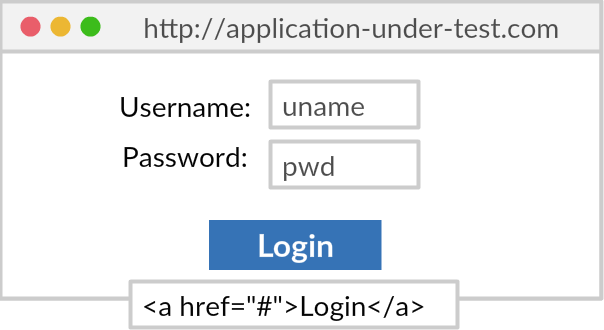
\includegraphics[width=5.6cm,height=2.8cm]{./Figures/newlogin}}
\vspace{-2mm}\subfigure[AUT version $V_{1}$]{\label{fig:3b}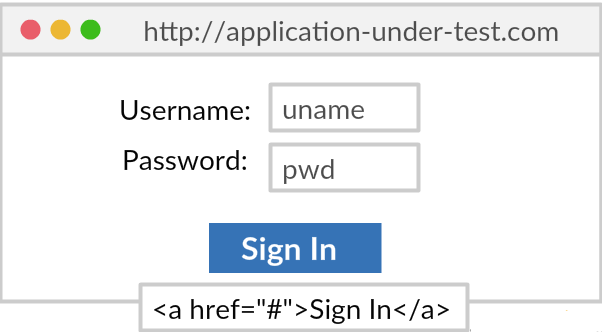
\includegraphics[width=5.6cm,height=2.8cm]{./Figures/newsignin}}
\caption{Evolution of the AUT from $V_{0}$ to $V_{1}$ breaks the fragile \texttt{loginTest} }
\label{fig:3loginTest}
\end{figure} 

In order to explore this issue, let us revisit the introductory example repeated here in Figure \ref{fig:3loginTest}. In this example, the \texttt{loginTest} uses \texttt{link text} locator for locating the ``Login'' button: \begin{small}
\texttt{driver.findElement(By.linkText("Login")).click()}
\end{small}
As the AUT evolves from version $V_{0}$ to $V_{1}$, the hyperlink text for ``Login'' button changes to ``Sign In''. This change does not alter the functionality of the AUT, rather its look-and-feel. According to the definition of robustness which we have developed in the penultimate section (Definition \ref{test-case-robustness}), a robust test should be able to explore the same functionality of the AUT regardless of the changes in the look-and-feel of the AUT. However in this example, \texttt{loginTest} is broken due to the the structural change and it cannot explore the \texttt{login} functionality of the AUT anymore. 

If the \texttt{loginTest} were to use a structure independent locator such as \texttt{id}, it would not have been susceptible to the renaming of ``Login'' button. Thus, choosing a suitable locator strategy plays a vital part for the robustness of the test. Each GUI locator differs in their characteristics such as availability and their susceptibility towards changes in GUI structure. A structure dependent locator is likely to be broken by minor changes in the application's GUI and needs to be repaired repeatedly if the AUT has frequent GUI changes. This process adds additional overhead in terms of the time required and costs incurred with the maintenance of the test-suite. The \textit{effort} of maintaining a test-suite can be measured in terms of the number of GUI locators repaired during two subsequent revisions $V_{0}$ and $V_{1}$ of the AUT. If developers know which type of locators are robust and do not need to be frequently repaired, they can improve their element location strategy to write more robust tests. 

To facilitate the maintenance of tests, the Page-object pattern (see Section \ref{page-object}) is helpful for the design of Selenium test-suites. This pattern provides a logical separation between the tests-code and the page-objects. Every time the test-suite needs to be repaired, e.g. changing the locator for ``Login'' button, only the \texttt{LoginPage} page-object needs to be changed as opposed to changing the locator for ``Login'' button in all tests. This minimizes the human error of forgetting to update a few tests. 


 
\chapter{Evaluation} % Main chapter title

\label{Chapter6} % For referencing the chapter elsewhere, use \ref{Chapter1} 

\lhead{Chapter 6. \emph{Approach and Evaluation}}
\chapter{Threats to validity} % Main chapter title

\label{Chapter7} % For referencing the chapter elsewhere, use \ref{Chapter1} 

\lhead{Chapter 7. \emph{Threats to validity}}
\chapter{Conclusion and Future Work} % Main chapter title

\label{Chapter7} % For referencing the chapter elsewhere, use \ref{Chapter1} 

\lhead{Chapter 7. \emph{Conclusion And Future Work}}

\section{Conclusion}
\label{conclusion}
An application's quality relies on continuous testing of its functionality while the success of the testing depends upon the robustness of the underlying tests. This thesis was able to formally define \textit{robustness} in the area of Selenium test automation and establish \textit{robustness grade} as a quantitative measurement for the robustness. 

The experimental results have shown that the Selenium tests are robust enough to stay functional during the first few new releases of an application. This leads to the conclusion that there are ways of prolonging the potential robustness level of the Selenium tests, although they will have to be repaired at some later point.

In addition, this thesis presented a set of metrics to establish which factors affect the robustness of Selenium tests the most and identified that none of the observed metrics solely is able to predict that the Selenium test will remain robust. Therefore, it can be concluded, after all, that a combination of certain metrics in the composition of particular tests definitely can contribute to robustness and may result in a less frequent maintenance process of the tests.

Overall, this research has successfully introduced and performed in practice one of the possible definitions for the robustness of Selenium tests and ways to measure it. This thesis can serve to developers as an additional source for handling the problems regarding the Selenium testing as well as to future researchers as a starting point for broadening the topic.
% In the area of automated regression testing using Selenium framework,  \textit{robustness} of a Selenium test implies the degree of its stability and effectiveness to cover the intended functionality across different versions of the application.




% During the development cycle of a web application, its features and functionalities are constantly being modified in order to maintain or improve its quality. Application's quality directly relies on continuous testing of its functioning and, in the end, results in desired performance at the GUI (Graphical User Interface) level appropriate for the users. The quality, therefore, depends upon testing while the success of the testing depends upon the robustness of the performed tests.

% Instead of manual testing, the developers often opt for automation of the whole process through Selenium framework. Selenium tests can be run automatically and repeatedly on an Application Under Test (AUT) as well as they would be later on rerun on the newer versions of the application in order to analyze its effectiveness. If the test has achieved the same functional coverage as it did for the original version it had been written for, the test can be considered \textit{robust}.

% The \textit{robustness} of a Selenium test implies the degree of its stability and effectiveness to cover the intended functionality across different versions of the AUT. It is numerically expressed through the \textit{robustness grade} in the interval [0,1], where a positive outcome indicates a robust test and any other a non-robust one. The research has been conducted on carefully picked open-source web application in order to determine how robust are Selenium tests against the changes of the AUT (RQ1), to determine if the robustness is correlated to the design and composition of the tests (RQ2) and if the design of the test-suite influence the maintenance effort (RQ3).


% The experimental results have shown that the tests are robust enough to stay functional during the first few new releases of an AUT which leads to the conclusion that there are ways of prolonging the potential robustness level although they will have to be repaired at some later point. Moreover, it has been seen that no specific metric in the design and composition of the test correlates directly with the robustness grade, however, we have also observed that compositions of some tests were more robust than the other ones. Therefore, it can be concluded, after all, that a combination of certain metrics in the composition of particular tests definitely can contribute to robustness.
% THIIIIIIIIIRRRDDD QQQQQQQQQQQQQQQQQQ CONCLUSION in short like previous ones.....

% The overall research has successfully introduced and performed in practice one of the possible definitions for the robustness of Selenium tests and ways to measure it. The thesis provides a concise overview of related works to this date about this topic and uses their conclusions to broaden it on a concrete level. The research has also, therefore, presented concrete results and problems which are to be expected when defining the robustness level of open-source applications' tests. The statistical analysis of the collected data has also resulted in defining a set of metrics which could potentially be considered as important contributors towards the robustness.

% The thesis can, therefore, serve as an additional source of handling the problems regarding the Selenium testing to developers as well as a starting point for broadening the topic to future researchers. 
% .................................. 


\newpage
\section{Future Work}
\label{futurework}
As this thesis is among the first ones of this kind, there are a many of ways in which the work presented in this research could be extended.

As mentioned in Chapter \ref{Chapter6}, the proposed approach is also transferable to other projects. Following this approach, the presented robustness metrics as well as maintenance metrics can be evaluated on other projects. From the presented metrics, the metrics \textit{\#partialLinkText},\textit{\#linkText} were not applicable in any project and hence their influence could not be studied. Given that majority of selected evaluation applications were industrial, it seems interesting to evaluate these metrics on applications and test-suites of different scales and development cycles to assess the outcome of the presented metrics. 

Furthermore, there are possibilities to include additional evaluation metrics in the research. It seems reasonable to apply the metrics this thesis was not able to cover. As an example, as a part of the \textit{\#waits} metric, only \texttt{implicitWait} and \texttt{SetTimeout} wait types were tested. Actions such as drag-drops, mouse-overs have also not been evaluated within this thesis. Additionally, in the area of Selenium testing for touch-enabled applications, the user-actions on such devices such as swipes, touch-gestures offers a richer set of metrics and hence it would be beneficial to assess them. 

In addition, for the metrics where no significant and consistent correlation could be estimated, as well as for reaching a concrete conclusion about the impact of the metrics, including larger sample size combined with more common metrics could improve the statistical results. 

% Overall, this thesis 


% % Chapter 1

\chapter{Chapter Title Here} % Main chapter title

\label{Chapter1} % For referencing the chapter elsewhere, use \ref{Chapter1} 

\lhead{Chapter 1. \emph{Chapter Title Here}} % This is for the header on each page - perhaps a shortened title

%----------------------------------------------------------------------------------------

\section{Welcome and Thank You}
Welcome to this \LaTeX{} Thesis Template, a beautiful and easy to use template for writing a thesis using the \LaTeX{} typesetting system.

If you are writing a thesis (or will be in the future) and its subject is technical or mathematical (though it doesn't have to be), then creating it in \LaTeX{} is highly recommended as a way to make sure you can just get down to the essential writing without having to worry over formatting or wasting time arguing with your word processor.

\LaTeX{} is easily able to professionally typeset documents that run to hundreds or thousands of pages long. With simple mark-up commands, it automatically sets out the table of contents, margins, page headers and footers and keeps the formatting consistent and beautiful. One of its main strengths is the way it can easily typeset mathematics, even \emph{heavy} mathematics. Even if those equations are the most horribly twisted and most difficult mathematical problems that can only be solved on a super-computer, you can at least count on \LaTeX{} to make them look stunning.

%----------------------------------------------------------------------------------------

\section{Learning \LaTeX{}}

\LaTeX{} is not a WYSIWYG (What You See is What You Get) program, unlike word processors such as Microsoft Word or Apple's Pages. Instead, a document written for \LaTeX{} is actually a simple, plain text file that contains \emph{no formatting}. You tell \LaTeX{} how you want the formatting in the finished document by writing in simple commands amongst the text, for example, if I want to use \textit{italic text for emphasis}, I write the `$\backslash$\texttt{textit}\{\}' command and put the text I want in italics in between the curly braces. This means that \LaTeX{} is a ``mark-up'' language, very much like HTML.

\subsection{A (not so short) Introduction to \LaTeX{}}

If you are new to \LaTeX{}, there is a very good eBook -- freely available online as a PDF file -- called, ``The Not So Short Introduction to \LaTeX{}''. The book's title is typically shortened to just ``lshort''. You can download the latest version (as it is occasionally updated) from here:\\
\href{http://www.ctan.org/tex-archive/info/lshort/english/lshort.pdf}{\texttt{http://www.ctan.org/tex-archive/info/lshort/english/lshort.pdf}}

It is also available in several other languages. Find yours from the list on this page:\\
\href{http://www.ctan.org/tex-archive/info/lshort/}{\texttt{http://www.ctan.org/tex-archive/info/lshort/}}

It is recommended to take a little time out to learn how to use \LaTeX{} by creating several, small `test' documents. Making the effort now means you're not stuck learning the system when what you \emph{really} need to be doing is writing your thesis.

\subsection{A Short Math Guide for \LaTeX{}}

If you are writing a technical or mathematical thesis, then you may want to read the document by the AMS (American Mathematical Society) called, ``A Short Math Guide for \LaTeX{}''. It can be found online here:\\
\href{http://www.ams.org/tex/amslatex.html}{\texttt{http://www.ams.org/tex/amslatex.html}}\\
under the ``Additional Documentation'' section towards the bottom of the page.

\subsection{Common \LaTeX{} Math Symbols}
There are a multitude of mathematical symbols available for \LaTeX{} and it would take a great effort to learn the commands for them all. The most common ones you are likely to use are shown on this page:\\
\href{http://www.sunilpatel.co.uk/latexsymbols.html}{\texttt{http://www.sunilpatel.co.uk/latexsymbols.html}}

You can use this page as a reference or crib sheet, the symbols are rendered as large, high quality images so you can quickly find the \LaTeX{} command for the symbol you need.

\subsection{\LaTeX{} on a Mac}
 
The \LaTeX{} package is available for many systems including Windows, Linux and Mac OS X. The package for OS X is called MacTeX and it contains all the applications you need -- bundled together and pre-customised -- for a fully working \LaTeX{} environment and workflow.
 
MacTeX includes a dedicated \LaTeX{} IDE (Integrated Development Environment) called ``TeXShop'' for writing your `\texttt{.tex}' files and ``BibDesk'': a program to manage your references and create your bibliography section just as easily as managing songs and creating playlists in iTunes.

%----------------------------------------------------------------------------------------

\section{Getting Started with this Template}

If you are familiar with \LaTeX{}, then you can familiarise yourself with the contents of the Zip file and the directory structure and then place your own information into the `\texttt{Thesis.cls}' file. Section \ref{FillingFile} on page \pageref{FillingFile} tells you how to do this. Make sure you read section \ref{ThesisConventions} about thesis conventions to get the most out of this template and then get started with the `\texttt{Thesis.tex}' file straightaway.

If you are new to \LaTeX{} it is recommended that you carry on reading through the rest of the information in this document.

\subsection{About this Template}

This \LaTeX{} Thesis Template is originally based and created around a \LaTeX{} style file created by Steve R.\ Gunn from the University of Southampton (UK), department of Electronics and Computer Science. You can find his original thesis style file at his site, here:\\
\href{http://www.ecs.soton.ac.uk/~srg/softwaretools/document/templates/}{\texttt{http://www.ecs.soton.ac.uk/$\sim$srg/softwaretools/document/templates/}}

My thesis originally used the `\texttt{ecsthesis.cls}' from his list of styles. However, I knew \LaTeX{} could still format better. To get the look I wanted, I modified his style and also created a skeleton framework and folder structure to place the thesis files in.

This Thesis Template consists of that modified style, the framework and the folder structure. All the work that has gone into the preparation and groundwork means that all you have to bother about is the writing.

Before you begin using this template you should ensure that its style complies with the thesis style guidelines imposed by your institution. In most cases this template style and layout will be suitable. If it is not, it may only require a small change to bring the template in line with your institution's recommendations.

%----------------------------------------------------------------------------------------

\section{What this Template Includes}

\subsection{Folders}

This template comes as a single Zip file that expands out to many files and folders. The folder names are mostly self-explanatory:

\textbf{Appendices} -- this is the folder where you put the appendices. Each appendix should go into its own separate `\texttt{.tex}' file. A template is included in the directory.

\textbf{Chapters} -- this is the folder where you put the thesis chapters. A thesis usually has about seven chapters, though there is no hard rule on this. Each chapter should go in its own separate `\texttt{.tex}' file and they usually are split as:
\begin{itemize}
\item Chapter 1: Introduction to the thesis topic
\item Chapter 2: Background information and theory
\item Chapter 3: (Laboratory) experimental setup
\item Chapter 4: Details of experiment 1
\item Chapter 5: Details of experiment 2
\item Chapter 6: Discussion of the experimental results
\item Chapter 7: Conclusion and future directions
\end{itemize}
This chapter layout is specialised for the experimental sciences.

\textbf{Figures} -- this folder contains all figures for the thesis. These are the final images that will go into the thesis document.

\textbf{Primitives} -- this is the folder that contains scraps, particularly because one final image in the `Figures' folder may be made from many separate images and photos, these source images go here. This keeps the intermediate files separate from the final thesis figures.

\subsection{Files}

Included are also several files, most of them are plain text and you can see their contents in a text editor. Luckily, many of them are auxiliary files created by \LaTeX{} or BibTeX and which you don't need to bother about:

\textbf{Bibliography.bib} -- this is an important file that contains all the bibliographic information and references that you will be citing in the thesis for use with BibTeX. You can write it manually, but there are reference manager programs available that will create and manage it for you. Bibliographies in \LaTeX{} are a large subject and you may need to read about BibTeX before starting with this.

\textbf{Thesis.cls} -- this is an important file. It is the style file that tells \LaTeX{} how to format the thesis. You will also need to open this file in a text editor and fill in your own information (such as name, department, institution). Luckily, this is not too difficult and is explained in section \ref{FillingFile} on page \pageref{FillingFile}.

\textbf{Thesis.pdf} -- this is your beautifully typeset thesis (in the PDF file format) created by \LaTeX{}.

\textbf{Thesis.tex} -- this is an important file. This is the file that you tell \LaTeX{} to compile to produce your thesis as a PDF file. It contains the framework and constructs that tell \LaTeX{} how to layout the thesis. It is heavily commented so you can read exactly what each line of code does and why it is there. After you put your own information into the `\texttt{Thesis.cls}' file, go to this file and begin filling it in -- you have now started your thesis!

\textbf{vector.sty} -- this is a \LaTeX{} package, it tells \LaTeX{} how to typeset mathematical vectors. Using this package is very easy and you can read the documentation on the site (you just need to look at the `\texttt{vector.pdf}' file):\\
\href{http://www.ctan.org/tex-archive/macros/latex/contrib/vector/}{\texttt{http://www.ctan.org/tex-archive/macros/latex/contrib/vector/}}

\textbf{lstpatch.sty} -- this is a \LaTeX{} package required by this LaTeX template and is included as not all \TeX{} distributions have it installed by default. You do not need to modify this file.

Files that are \emph{not} included, but are created by \LaTeX{} as auxiliary files include:

\textbf{Thesis.aux} -- this is an auxiliary file generated by \LaTeX{}, if it is deleted \LaTeX{} simply regenerates it when you run the main `\texttt{.tex}' file.

\textbf{Thesis.bbl} -- this is an auxiliary file generated by BibTeX, if it is deleted, BibTeX simply regenerates it when you run the main tex file. Whereas the `\texttt{.bib}' file contains all the references you have, this `\texttt{.bbl}' file contains the references you have actually cited in the thesis and is used to build the bibliography section of the thesis.

\textbf{Thesis.blg} -- this is an auxiliary file generated by BibTeX, if it is deleted BibTeX simply regenerates it when you run the main `\texttt{.tex}' file.

\textbf{Thesis.lof} -- this is an auxiliary file generated by \LaTeX{}, if it is deleted \LaTeX{} simply regenerates it when you run the main `\texttt{.tex}' file. It tells \LaTeX{} how to build the `List of Figures' section.

\textbf{Thesis.log} -- this is an auxiliary file generated by \LaTeX{}, if it is deleted \LaTeX{} simply regenerates it when you run the main `\texttt{.tex}' file. It contains messages from \LaTeX{}, if you receive errors and warnings from \LaTeX{}, they will be in this `\texttt{.log}' file.

\textbf{Thesis.lot} -- this is an auxiliary file generated by \LaTeX{}, if it is deleted \LaTeX{} simply regenerates it when you run the main `\texttt{.tex}' file. It tells \LaTeX{} how to build the `List of Tables' section.

\textbf{Thesis.out} -- this is an auxiliary file generated by \LaTeX{}, if it is deleted \LaTeX{} simply regenerates it when you run the main `\texttt{.tex}' file.


So from this long list, only the files with the `\texttt{.sty}', `\texttt{.bib}', `\texttt{.cls}' and `\texttt{.tex}' extensions are the most important ones. The other auxiliary files can be ignored or deleted as \LaTeX{} and BibTeX will regenerate them.

%----------------------------------------------------------------------------------------

\section{Filling in the `\texttt{Thesis.cls}' File}\label{FillingFile}

You will need to personalise the thesis template and make it your own by filling in your own information. This is done by editing the `\texttt{Thesis.cls}' file in a text editor.

Open the file and scroll down, past all the `$\backslash$\texttt{newcommand}\ldots' items until you see the entries for `\texttt{University Name}', `\texttt{Department Name}', etc\ldots.

Fill out the information about your group and institution and ensure you keep to block capitals where it asks you to. You can also insert web links, if you do, make sure you use the full URL, including the `\texttt{http://}' for this.

The last item you should need to fill in is the Faculty Name (in block capitals). When you have done this, save the file and recompile `\texttt{Thesis.tex}'. All the information you filled in should now be in the PDF, complete with web links. You can now begin your thesis proper!

%----------------------------------------------------------------------------------------

\section{The `\texttt{Thesis.tex}' File Explained}

The \texttt{Thesis.tex} file contains the structure of the thesis. There are plenty of written comments that explain what pages, sections and formatting the \LaTeX{} code is creating. Initially there seems to be a lot of \LaTeX{} code, but this is all formatting, and it has all been taken care of so you don't have to do it.

Begin by checking that your information on the title page is correct. For the thesis declaration, your institution may insist on something different than the text given. If this is the case, just replace what you see with what is required.

Then comes a page which contains a funny quote. You can put your own, or quote your favourite scientist, author, person, etc\ldots Make sure to put the name of the person who you took the quote from.

Next comes the acknowledgements. On this page, write about all the people who you wish to thank (not forgetting parents, partners and your advisor/supervisor).

The contents pages, list of figures and tables are all taken care of for you and do not need to be manually created or edited. The next set of pages are optional and can be deleted since they are for a more technical thesis: insert a list of abbreviations you have used in the thesis, then a list of the physical constants and numbers you refer to and finally, a list of mathematical symbols used in any formulae. Making the effort to fill these tables means the reader has a one-stop place to refer to instead of searching the internet and references to try and find out what you meant by certain abbreviations or symbols.

The list of symbols is split into the Roman and Greek alphabets. Whereas the abbreviations and symbols ought to be listed in alphabetical order (and this is \emph{not} done automatically for you) the list of physical constants should be grouped into similar themes.

The next page contains a one line dedication. Who will you dedicate your thesis to?

Finally, there is the section where the chapters are included. Uncomment the lines (delete the `\texttt{\%}' character) as you write the chapters. Each chapter should be written in its own file and put into the `Chapters' folder and named `\texttt{Chapter1}', `\texttt{Chapter2}, etc\ldots Similarly for the appendices, uncomment the lines as you need them. Each appendix should go into its own file and placed in the `Appendices' folder.

After the preamble, chapters and appendices finally comes the bibliography. The bibliography style (called `\texttt{unsrtnat}') is used for the bibliography and is a fully featured style that will even include links to where the referenced paper can be found online. Do not under estimate how grateful you reader will be to find that a reference to a paper is just a click away. Of course, this relies on you putting the URL information into the BibTeX file in the first place.

%----------------------------------------------------------------------------------------

\section{Thesis Features and Conventions}\label{ThesisConventions}

To get the best out of this template, there are a few conventions that you may want to follow.

One of the most important (and most difficult) things to keep track of in such a long document as a thesis is consistency. Using certain conventions and ways of doing things (such as using a Todo list) makes the job easier. Of course, all of these are optional and you can adopt your own method.

\subsection{Printing Format}

This thesis template is designed for single sided printing as most theses are printed and bound this way. This means that the left margin is always wider than the right (for binding). Four out of five people will now judge the margins by eye and think, ``I never 
noticed that before.''.

The headers for the pages contain the page number on the right side (so it is easy to flick through to the page you want) and the chapter name on the left side.

The text is set to 11 point and a line spacing of 1.3. Generally, it is much more readable to have a smaller text size and wider gap between the lines than it is to have a larger text size and smaller gap. Again, you can tune the text size and spacing should you want or need to. The text size can be set in the options for the `$\backslash$\texttt{documentclass}' command at the top of the `\texttt{Thesis.tex}' file and the spacing can be changed by setting a different value in the `$\backslash$\texttt{setstretch}' commands (scattered throughout the `\texttt{Thesis.tex}' file).

\subsection{Using US Letter Paper}

The paper size used in the template is A4, which is a common -- if not standard -- size in Europe. If you are using this thesis template elsewhere and particularly in the United States, then you may have to change the A4 paper size to the US Letter size. Unfortunately, this is not as simple as replacing instances of `\texttt{a4paper}' with `\texttt{letterpaper}'.

This is because the final PDF file is created directly from the \LaTeX{} source using a program called `\texttt{pdfTeX}' and in certain conditions, paper size commands are ignored and all documents are created with the paper size set to the size stated in the configuration file for pdfTeX (called `\texttt{pdftex.cfg}').

What needs to be done is to change the paper size in the configuration file for \texttt{pdfTeX} to reflect the letter size. There is an excellent tutorial on how to do this here: \\
\href{http://www.physics.wm.edu/~norman/latexhints/pdf_papersize.html}{\texttt{http://www.physics.wm.edu/$\sim$norman/latexhints/pdf\_papersize.html}}

It may be sufficient just to replace the dimensions of the A4 paper size with the US Letter size in the \texttt{pdftex.cfg} file. Due to the differences in the paper size, the resulting margins may be different to what you like or require (as it is common for Institutions to dictate certain margin sizes). If this is the case, then the margin sizes can be tweaked by opening up the \texttt{Thesis.cls} file and searching for the line beginning with, `$\backslash$\texttt{setmarginsrb}' (not very far down from the top), there you will see the margins specified. Simply change those values to what you need (or what looks good) and save. Now your document should be set up for US Letter paper size with suitable margins.

\subsection{References}

The `\texttt{natbib}' package is used to format the bibliography and inserts references such as this one \citep{Reference3}. The options used in the `\texttt{Thesis.tex}' file mean that the references are listed in numerical order as they appear in the text. Multiple references are rearranged in numerical order (e.g. \citep{Reference2, Reference1}) and multiple, sequential references become reformatted to a reference range (e.g. \citep{Reference2, Reference1, Reference3}). This is done automatically for you. To see how you use references, have a look at the `\texttt{Chapter1.tex}' source file. Many reference managers allow you to simply drag the reference into the document as you type.

Scientific references should come \emph{before} the punctuation mark if there is one (such as a comma or period). The same goes for footnotes\footnote{Such as this footnote, here down at the bottom of the page.}. You can change this but the most important thing is to keep the convention consistent throughout the thesis. Footnotes themselves should be full, descriptive sentences (beginning with a capital letter and ending with a full stop).

To see how \LaTeX{} typesets the bibliography, have a look at the very end of this document (or just click on the reference number links).

\subsection{Figures}

There will hopefully be many figures in your thesis (that should be placed in the `Figures' folder). The way to insert figures into your thesis is to use a code template like this:
\begin{verbatim}
\begin{figure}[htbp]
  \centering
    
\includegraphics{./Figures/Electron.pdf}
    \rule{35em}{0.5pt}
  \caption[An Electron]{An electron (artist's impression).}
  \label{fig:Electron}
\end{figure}
\end{verbatim}
Also look in the source file. Putting this code into the source file produces the picture of the electron that you can see in the figure below.

\begin{figure}[htbp]
	\centering
		
\includegraphics{./Figures/Electron.pdf}
		\rule{35em}{0.5pt}
	\caption[An Electron]{An electron (artist's impression).}
	\label{fig:Electron}
\end{figure}

Sometimes figures don't always appear where you write them in the source. The placement depends on how much space there is on the page for the figure. Sometimes there is not enough room to fit a figure directly where it should go (in relation to the text) and so \LaTeX{} puts it at the top of the next page. Positioning figures is the job of \LaTeX{} and so you should only worry about making them look good!

Figures usually should have labels just in case you need to refer to them (such as in Figure \ref{fig:Electron}). The `$\backslash$\texttt{caption}' command contains two parts, the first part, inside the square brackets is the title that will appear in the `List of Figures', and so should be short. The second part in the curly brackets should contain the longer and more descriptive caption text.

The `$\backslash$\texttt{rule}' command is optional and simply puts an aesthetic horizontal line below the image. If you do this for one image, do it for all of them.

The \LaTeX{} Thesis Template is able to use figures that are either in the PDF or JPEG file format.

\subsection{Typesetting mathematics}

If your thesis is going to contain heavy mathematical content, be sure that \LaTeX{} will make it look beautiful, even though it won't be able to solve the equations for you.

The ``Not So Short Introduction to \LaTeX{}'' (available \href{http://www.ctan.org/tex-archive/info/lshort/english/lshort.pdf}{here}) should tell you everything you need to know for most cases of typesetting mathematics. If you need more information, a much more thorough mathematical guide is available from the AMS called, ``A Short Math Guide to \LaTeX{}'' and can be downloaded from:\\
\href{ftp://ftp.ams.org/pub/tex/doc/amsmath/short-math-guide.pdf}{\texttt{ftp://ftp.ams.org/pub/tex/doc/amsmath/short-math-guide.pdf}}

There are many different \LaTeX{} symbols to remember, luckily you can find the most common symbols \href{http://www.sunilpatel.co.uk/latexsymbols.html}{here}. You can use the web page as a quick reference or crib sheet and because the symbols are grouped and rendered as high quality images (each with a downloadable PDF), finding the symbol you need is quick and easy.

You can write an equation, which is automatically given an equation number by \LaTeX{} like this:
\begin{verbatim}
\begin{equation}
E = mc^{2}
  \label{eqn:Einstein}
\end{equation}
\end{verbatim}

This will produce Einstein's famous energy-matter equivalence equation:
\begin{equation}
E = mc^{2}
\label{eqn:Einstein}
\end{equation}

All equations you write (which are not in the middle of paragraph text) are automatically given equation numbers by \LaTeX{}. If you don't want a particular equation numbered, just put the command, `$\backslash$\texttt{nonumber}' immediately after the equation.

%----------------------------------------------------------------------------------------

\section{Sectioning and Subsectioning}

You should break your thesis up into nice, bite-sized sections and subsections. \LaTeX{} automatically builds a table of Contents by looking at all the `$\backslash$\texttt{chapter}$\{\}$', `$\backslash$\texttt{section}$\{\}$' and `$\backslash$\texttt{subsection}$\{\}$' commands you write in the source.

The table of Contents should only list the sections to three (3) levels. A `$\backslash$\texttt{chapter}$\{\}$' is level one (1). A `$\backslash$\texttt{section}$\{\}$' is level two (2) and so a `$\backslash$\texttt{subsection}$\{\}$' is level three (3). In your thesis it is likely that you will even use a `$\backslash$\texttt{subsubsection}$\{\}$', which is level four (4). Adding all these will create an unnecessarily cluttered table of Contents and so you should use the `$\backslash$\texttt{subsubsection$^{*}\{\}$}' command instead (note the asterisk). The asterisk ($^{*}$) tells \LaTeX{} to omit listing the subsubsection in the Contents, keeping it clean and tidy.

%----------------------------------------------------------------------------------------

\section{In Closing}

You have reached the end of this mini-guide. You can now rename or overwrite this pdf file and begin writing your own `\texttt{Chapter1.tex}' and the rest of your thesis. The easy work of setting up the structure and framework has been taken care of for you. It's now your job to fill it out!

Good luck and have lots of fun!

\begin{flushright}
Guide written by ---\\
Sunil Patel: \href{http://www.sunilpatel.co.uk}{www.sunilpatel.co.uk}
\end{flushright}

%----------------------------------------------------------------------------------------
%	THESIS CONTENT - APPENDICES
%----------------------------------------------------------------------------------------

\addtocontents{toc}{\vspace{2em}} % Add a gap in the Contents, for aesthetics

\appendix % Cue to tell LaTeX that the following 'chapters' are Appendices

% Include the appendices of the thesis as separate files from the Appendices folder
% Uncomment the lines as you write the Appendices

% Appendix A

\chapter{Versioning for Web Applications} % Main appendix title

\label{AppendixA} % For referencing this appendix elsewhere, use \ref{AppendixA}

\lhead{Appendix A. \emph{Major and minor versions for selected applications}} % This is for the header on each page - perhaps a shortened title
% \end{savenotes}

\begin{table}[h!]
\parbox{.5\linewidth}{
\centering
\begin{tabular}{l*{1}{l}r}
\hline
Version (\texttt{git tag}) \\
\hline
2014.12.16      \\
2014.12.22-02   \\
2015.01.06      \\
2015.01.20      \\
2015.01.27      \\
2015.02.10      \\
2015.02.24      \\
2015.03.10      \\
2015.04.01      \\
2015.04.10      \\
2015.04.21      \\
2015.04.28      \\
2015.07.07      \\
2015.07.07      \\
2015.07.21      \\
2015.07.31      \\
2015.08.11      \\
2015.08.25      \\
2015.09.08      \\
2015.09.22      \\
2015.09.29      \\
2015.10.13      \\
2015.11.02      \\
2015.11.02      \\
2015.11.17      \\
2015.11.24      \\
2015.12.01      \\
2015.12.22      \\
2016.01.12 \\

\hline
\end{tabular}
\caption{Mozilla Marketplace}
\label{fireplace}
}
\hfill
\parbox{.45\linewidth}{
\centering
\begin{tabular}{l*{1}{l}r}
\hline
Version (\texttt{git tag}) \\
\hline
1.580 \\
1.582 \\
1.584 \\
1.586 \\
1.588 \\
1.590 \\
1.592 \\
1.594 \\
1.596 \\
1.598 \\
1.600 \\
1.602 \\
1.604 \\
1.606 \\
1.608 \\
1.609 \\
1.611 \\
1.613 \\
1.615 \\
1.617 \\
1.619 \\
1.621 \\
1.623 \\
1.625 \\
1.627 \\
1.629 \\
1.631 \\
1.633 \\
1.635 \\

\hline
\end{tabular}
\caption{Jenkins}
\label{jenkins}

}

\end{table}

\begin{table}[h!]
\parbox{.5\linewidth}{
\centering
\begin{tabular}{l*{1}{l}r}
\hline
Version (\texttt{git tag}) \\
\hline
2.3 \\
2.3.1	\\
2.3.2	\\
2.3.3	\\
2.3.4	\\
2.3.5	\\
2.3.6	\\
2.3.7	\\
2.3.8	\\
2.3.9	\\
2.3.10 \\
2.3.11 \\
\hline
\end{tabular}
\caption{Moodle}
\label{moodle}
}
\parbox{.5\linewidth}{
\centering
\begin{tabular}{l*{1}{l}r}
\hline
Version (\texttt{git tag}) \\
\hline
2015.01.13    \\
2015.01.21    \\
2015.01.30    \\
2015.02.13    \\
2015.02.26    \\
2015.03.12    \\
2015.03.21    \\
2015.03.30    \\
2015.04.10    \\
2015.04.20    \\
2015.04.30    \\
2015.05.11    \\
2015.05.27    \\
2015.06.08    \\
2015.06.15    \\
2015.07.01    \\
2015.07.15    \\
2015.07.31    \\
2015.08.14    \\
2015.09.16    \\
2015.10.01    \\
2015.10.15    \\
2015.10.26    \\
\hline
\end{tabular}
\caption{Mozilla Addons}
\label{amo}
}
\hfill
\parbox{.45\linewidth}{
\centering
\begin{tabular}{l*{1}{l}r}
% \centering
\hline
Version (\texttt{git commit})  \\
\hline
25dc8adfebedb22eb900fae1e083b5767bc6223e \\
2c8024b2a4d97d3d6831ff21620bb399b41afee3  \\
4be52ca79504431a202270201848e636e01b22cb \\
bdf4422b2ba17d8e05c3776343cad65974184163 \\
1ab227632b6d2b3a9cf2d4834656117e3a38f8ea \\
f6e89fd4d1d4e5116e70c63026ce66419e898221 \\
5635154584ca3efb29cc0fc3924d5d9ee924062b  \\
889acbcf37c0447b9a05eb3dfb18e1d52ae347b3 \\
1b1a295c08fb6bc39fe72e33001cb03f5ed0ab09  \\
06afb836430101fc5af8b163f0ef50ca58cdbed8  \\
8c58e496d98deb39fed707334251e7276972f56a  \\
74779d29aeae26da581fc1a65ec5c425cf64e0c5 \\
77fffdc3cd0658199ac01657bda612ff8eb42fc7  \\
14f19f2182a0ae004ad0b4043b07e4e58c208d78 \\
9759b494e547bf191430f2c7ddd0047b31aac67a \\
044436b2e456aa1624830c8e846a9e60c99f911e \\
c3431b7378a51d53cc4f4606fbe1dc8744707b1b  \\
88fc9535a46284616d0f10d01dedc88b4a1e99a8 \\
6217987286a9af00a52e1750f219840e09544a61 \\ 
\hline
\end{tabular}
\caption{Mozilla.org}
\label{bedrock}

}

\end{table}
% Appendix A

\chapter{List of test-suite commits} % Main appendix title

\label{AppendixB} % For referencing this appendix elsewhere, use \ref{AppendixA}

\lhead{Appendix B. \emph{Test suite reference commits}} % This is for the header on each page - perhaps a shortened title

Write your Appendix content here.
%\input{./Appendices/AppendixC}

\addtocontents{toc}{\vspace{2em}} % Add a gap in the Contents, for aesthetics

\backmatter

%----------------------------------------------------------------------------------------
%	BIBLIOGRAPHY
%----------------------------------------------------------------------------------------

\label{Bibliography}

\lhead{\emph{Bibliography}} % Change the page header to say "Bibliography"

\bibliographystyle{unsrtnat} % Use the "unsrtnat" BibTeX style for formatting the Bibliography

\bibliography{Bibliography} % The references (bibliography) information are stored in the file named "Bibliography.bib"

\end{document}